\documentclass[oneside, a4paper, 12pt]{report}

\usepackage{ngerman}
\usepackage{graphicx}
\usepackage{xcolor}
\usepackage[T1]{fontenc}
\usepackage[latin1]{inputenc}
\usepackage{lmodern}
\usepackage{geometry}
\usepackage[numbers]{natbib}
\usepackage[pagestyles]{titlesec}
\usepackage{titletoc}
\usepackage{microtype}
\usepackage{booktabs}
\usepackage{caption}
\usepackage{subcaption}
\usepackage{setspace}
\usepackage{calc}
\usepackage[colorlinks]{hyperref}
\usepackage{amsmath,amsfonts,amssymb,amsthm}
\usepackage{mathtools}
\usepackage[version=3]{mhchem}
\usepackage{wrapfig}
\usepackage{tikz}
\usepackage{cancel}
\usepackage{algorithm}
\usepackage{algpseudocode}
\usepackage{url}

\DeclarePairedDelimiter\ceil{\lceil}{\rceil}
\DeclarePairedDelimiter\floor{\lfloor}{\rfloor}

\renewcommand\abstractname{Vorwort}

% Layout der "Uberschriften
\titleformat{\chapter}[hang]
{\fontfamily{pag}\Large\bfseries}{\thechapter}{1.5cm-\widthof{\thechapter}}{\large\bfseries}
\titleformat{\section}
{\fontfamily{pag}\normalsize\bfseries}{\thesection}{1.5cm-\widthof{\thesection}}{\normalsize}
\titleformat{\subsection}
{\fontfamily{pag}\normalsize\bfseries}{\thesubsection}{1.5cm-\widthof{\thesubsection}}{\normalsize} 

% Seitenlayout (Kopf und Fu"szeile)
\newpagestyle{mystyle}
{
	\headrule
	\sethead{\thechapter. \chaptertitle}{}{\thepage}
	%
	\footrule
	\setfoot{\textnormal{Android}}\raggedleft{\textnormal{Christoph Weik}}
} 

\pagestyle{mystyle}
\parindent0pt
\onehalfspacing
\geometry{outer=20mm,  inner=25mm,  top=20mm,  bottom=30mm}

\begin{document}
	\begin{titlepage}
		%
		\begin{flushleft}
			
\includegraphics[width=0.35\textwidth]{android_title.jpg}
		\end{flushleft}
		%
		\vspace*{3.5cm}
		\begin{center}
			\Huge{\bf PiSense mit Quadrocopter 2016\bigskip\bigskip\\}
			\LARGE{Android Applikation\\ Fernsteuerung\bigskip\bigskip\\}
			\large{Uni T�bingen\vfill}
		\end{center}
		%
		\vspace*{1cm}
		\begin{minipage}{\widthof{Christoph Weik}}
			\begin{flushleft}
				Author:\\
				Christoph Weik
			\end{flushleft}
		\end{minipage}
		\hfill
		\begin{minipage}{\widthof{\today}}
			\begin{flushright}
				Dienstag 20.08.16
			\end{flushright}
		\end{minipage}
	\end{titlepage}
	%
	\newpage
	\begin{abstract}
		\centering
		In allen Informatikstudieng"angen der Universit"at T"ubingen ist die Teilnahme an einem Softwareprojekt verpflichtend. Das Team-Projekt PiSense mit Quadrocopter, handelte rund um die Anpassung der Low-Level-Treiber, um  das Speichern sowie Auslesen von Sensordaten in Datenbank und GUI zu erm"oglichen. Der folgenden Unterabschnitt des Projekts hatte zum Ziel, die Entwicklung einer Applikation zur Steuerung der Rotorgeschwindigkeit und Senden vorgegebener Befehlsketten an den Raspberry Pi. Diese wurde von Grund auf neu entworfen und beruht nicht auf Arbeiten vorheriger Semester.
	\end{abstract}
	%
	\newpage
	%Inhalts-, Abbildungs-, und Tabellenverzeichnis
	\pagenumbering{Roman}
	\begingroup
	\let\clearpage\relax
	\tableofcontents
	\listoffigures
	\endgroup
	%
	\newpage
	\pagenumbering{arabic}
	\chapter{Getting Started (mit Windows 7)}
		\section{Java 8 installieren}
			\subsection{Installation des Java Development Kit 8}
			Die aktuellste Version des JDK findet man auf der Herstellerwebsite unter:
			\begin{itemize}
				\item \url{http://www.oracle.com/technetwork/java/javase/downloads/index.html}
			\end{itemize}
			%
			\begin{figure}[h!]
				\centering
				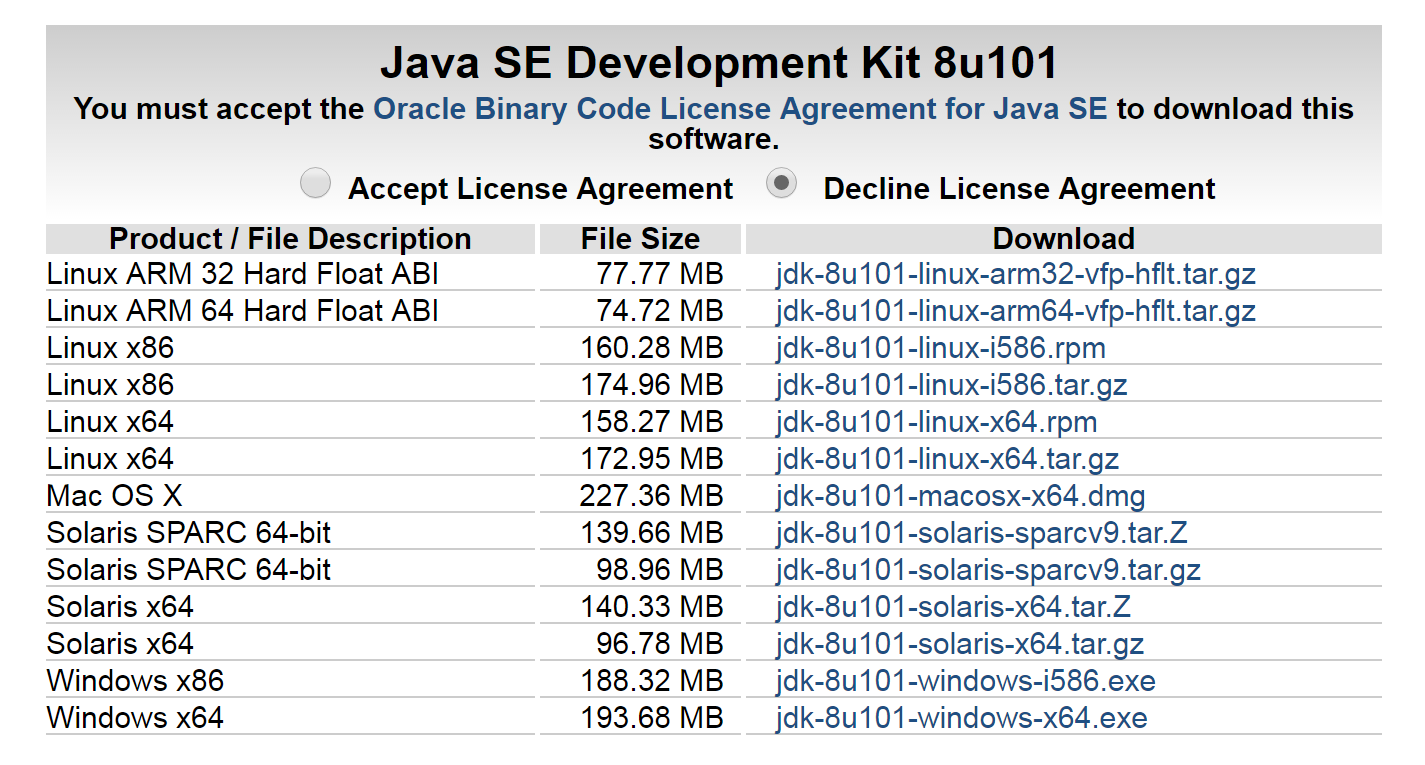
\includegraphics[width=0.8\textwidth]{jdk_download.png}
				\caption{Aktuelle Portierungen des JDK 8. \label{jdk_dl}}
			\end{figure}
			%
			Die ben"otigte Java-Installationsdatei hei�t im Falle von Microsoft Windows 7 (64 Bit) jdk-8u101-windows-x64.exe.
			\\ \newline
			Vor der Installation ist es jedoch sinnvoll zu Pr"ufen, ob bereits die aktuellste Version vorliegt. Die geschieht in Windows 7 folgenderma"sen:
			\begin{itemize}
				\item[1.] "Offne zuerst die Kommandozeile (Windowstaste + R $\to$ im Eingabefeld \textbf{cmd} eingeben).
				\item[2.] In der Kommandozeile \textbf{java -version} eingeben.
			\end{itemize}
			%
			\newpage
			\begin{figure}[h!]
				\centering
				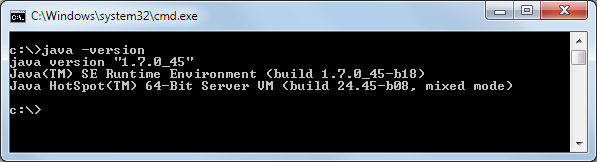
\includegraphics[width=0.8\textwidth]{java_8_installieren_version_pruefen.png}
				\caption{Ausgabe der aktuell installierten Java Version in der Kommandozeile. \label{cmdJava}}
			\end{figure}
			%
			In diesem Beispiel ist die Java Version 1.7.0\_45 bereits veraltet und eine neuere Version sollte installiert werden.
			%
			\subsection{Installation der Java-Dokumentation}
			Die folgenden Links f�hren zur Online Dokumentation von Java 8 SE und der Download-Seite:
			\begin{itemize}
				\item \url{http://docs.oracle.com/javase/8/docs/index.html}
				\item \url{http://www.oracle.com/technetwork/java/javase/documentation/jdk8-doc-downloads-2133158.html}
			\end{itemize}
			%
			F"ur uns ist nur die obere mit der Bezeichnung  \glqq Java SE Development Kit 8u101 Documentation\grqq~ relevant. Diese entpacken wir und kopieren sie anschlie"send in das JDK-Verzeichnis.
			\begin{figure}[h!]
				\centering
				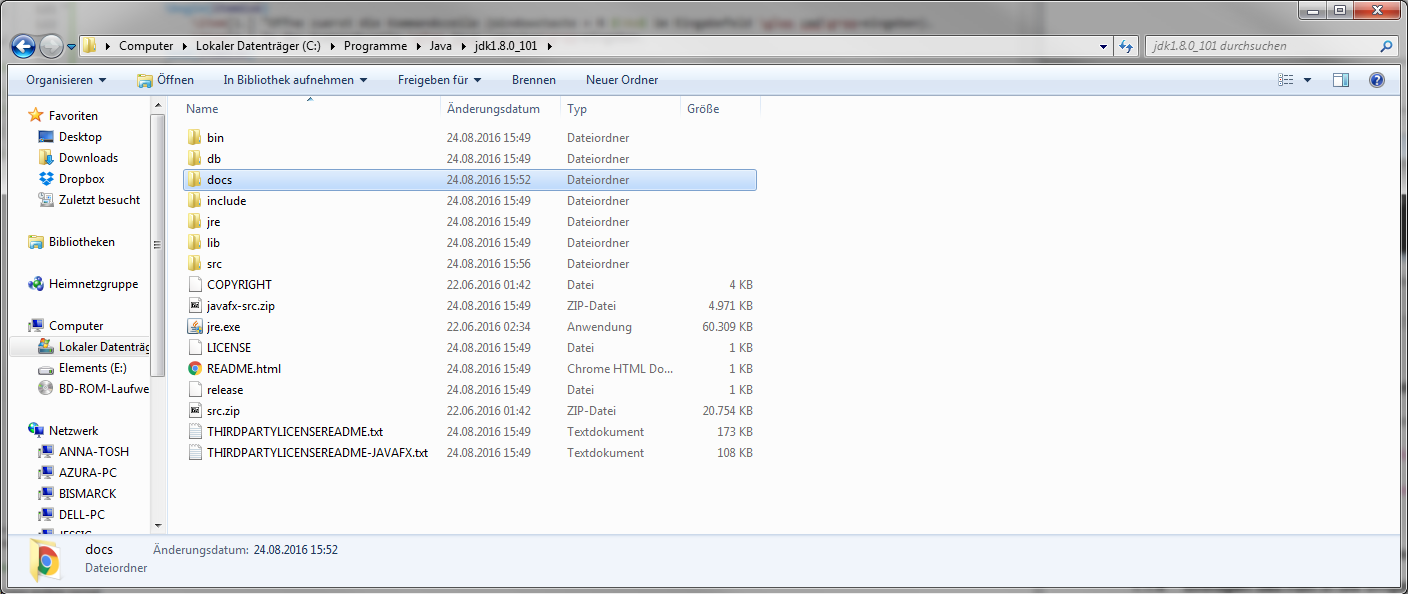
\includegraphics[width=\textwidth]{java_docs.png}
				\caption{Kopieren des Docs-Verzeichnis in das JDK-Verzeichnis. \label{docsJava}}
			\end{figure}
			%
			\newpage
			Die Java-Dokumentation wird �ber einen Browser betrachtet. Es bietet sich daher an ein Lesezeichen anzulegen, welches auf das Hauptdokument verweist. Wie bspw.:\\
			\path{file://localhost/C:/Program%20Files/Java/jdk1.8.0_101/docs/index.html}
			\begin{figure}[h!]
				\centering
				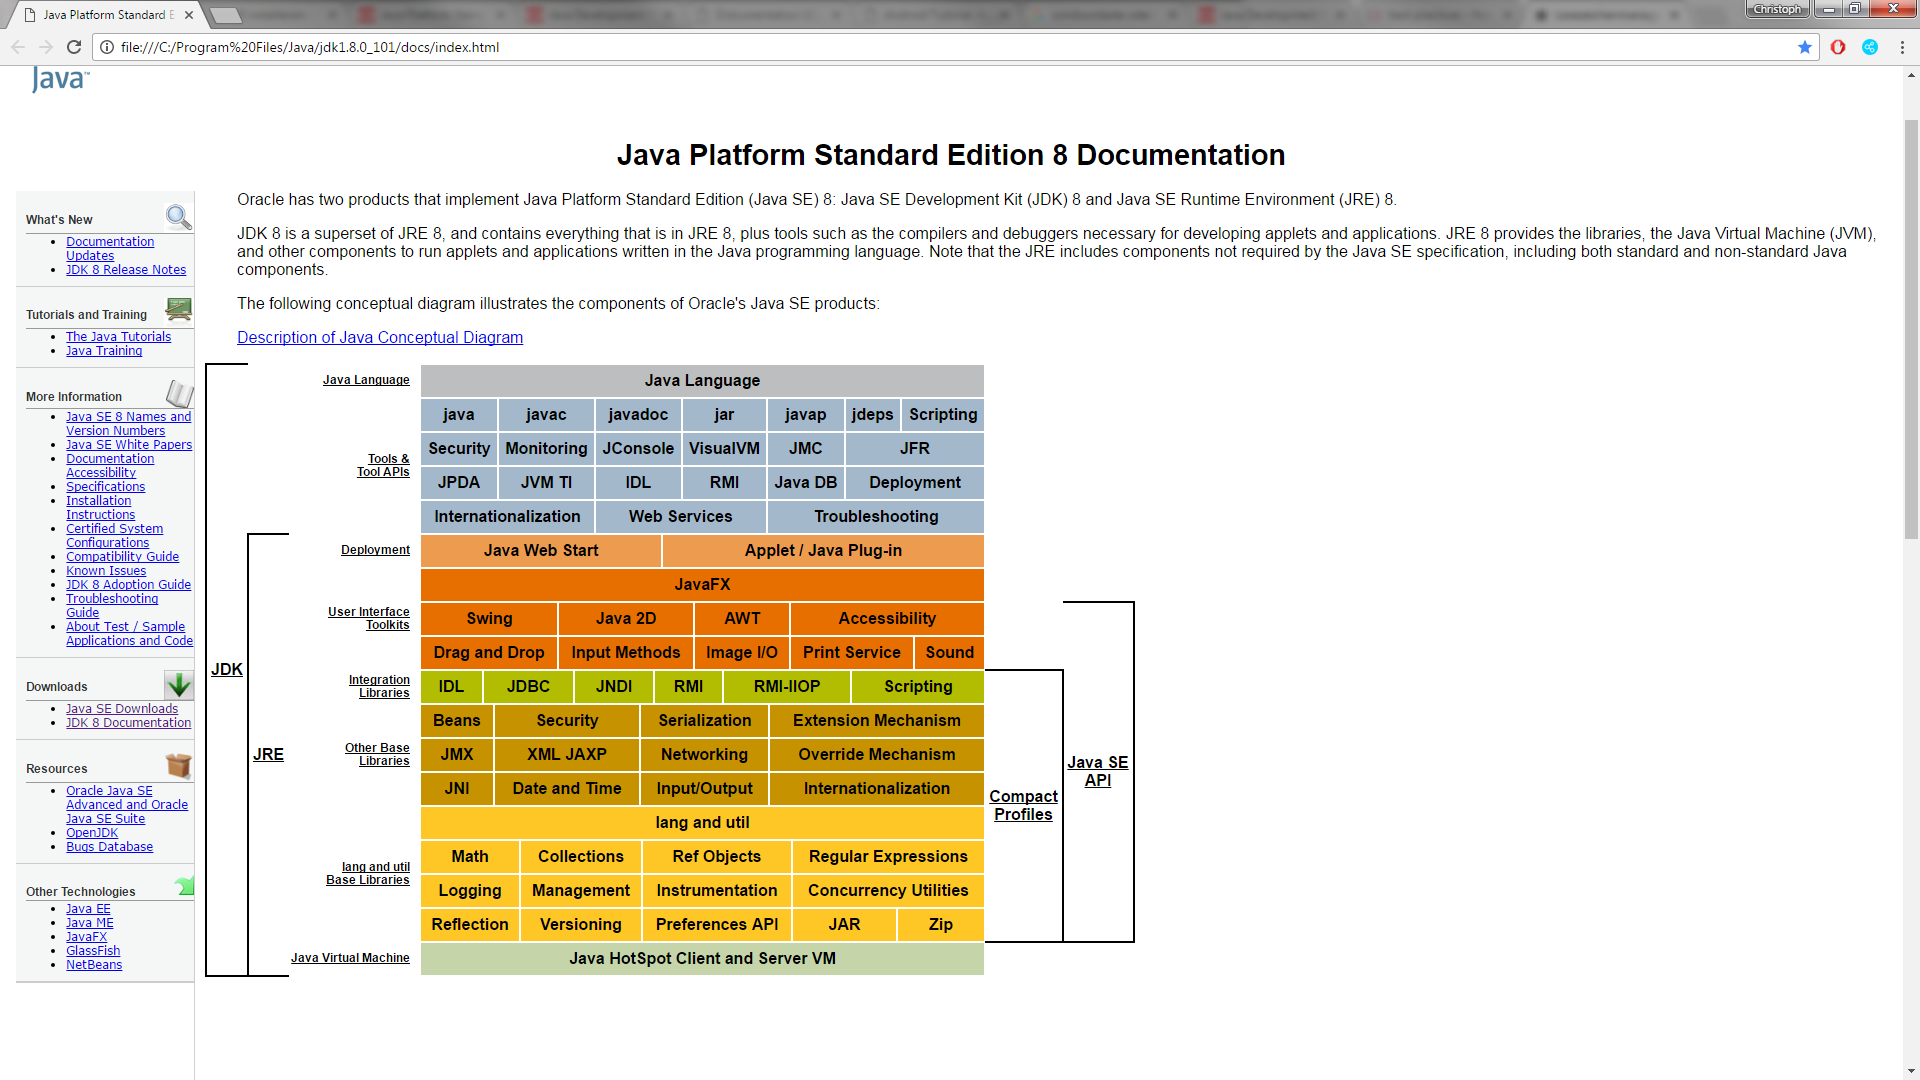
\includegraphics[width=0.8\textwidth]{java_lesezeichen.png}
				\caption{Lesezeichen Dokumentation Java 8 SE. \label{lzJava}}
			\end{figure}
			%
			\subsection{Installation der Java-Quelltexte}
			Die Quelltexte befinden sich bereits im Installationsverzeichnis des  JDK 8 und m"ussen nur noch entpackt werden.
			\begin{figure}[h!]
				\centering
				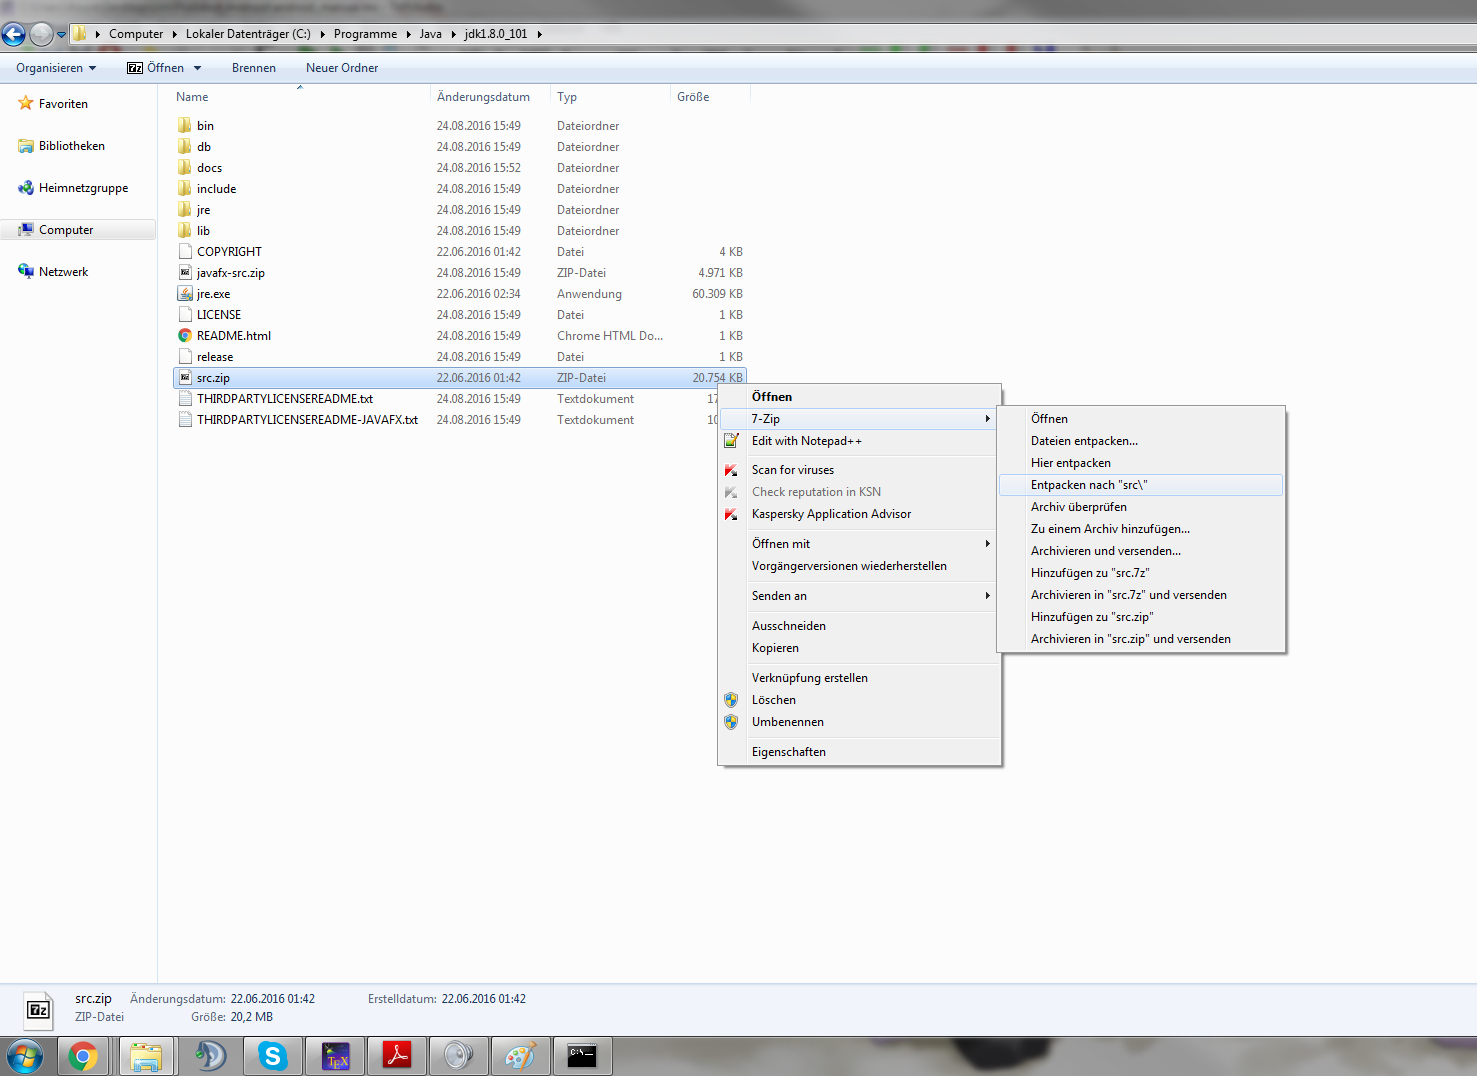
\includegraphics[width=0.75\textwidth]{java_quelltext.png}
				\caption{Entpacken der Archivdatei. \label{qtJava}}
			\end{figure}
			%
			\newpage
			\subsection{Eintragen des Path in die Umgebungsvariable}
			Unter Windows 7 kann die Systemvariable Path folgenderma"sen ge"andert werden:
			\begin{itemize}
				\item[1.] Windowstaste + Pause, dann erweiterte Systemeinstellungen.
				\item[2.] Auf dem Reiter Erweitert w"ahlen wir Umgebungsvariablen\dots.
				\item[3.] F"uge den Pfad des bin-Ordners der JDK-Installation in die Systemvariable Path ein.
			\end{itemize}
			%
			Die Path Variable k"onnte dann beispielsweise so aussehen:\\
			\path{C:\WINDOWS\system32;C:\WINDOWS;C:\Program Files\Java\jdk1.8.0_101\bin}\\
			Nun sollte es auch m"oglich sein durch den Befehl \textbf{javac -version} die Version des Java Compilers auszugeben.
			\begin{figure}[h!]
				\centering
				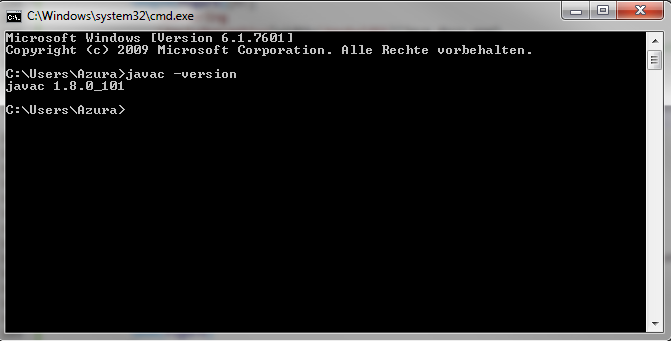
\includegraphics[width=0.8\textwidth]{javac_cmd.png}
				\caption{Ausgeben der Versionsnummer des Java Compilers. \label{javac}}
			\end{figure}
			%
		\newpage
		\section{Android Studio installieren}
			\subsection{Installation des Hauptprogramms}
			Die Installationsdatei von Android Studio findet ihr auf der Android Entwickler Webseite. "Uber die Reiter Develop > Android Studio gelangt ihr zum Download-Bereich.
			\begin{itemize}
				\item \url{http://developer.android.com/}
			\end{itemize}
			%
			Nach dem Starten des Wizards werdet ihr kurze Zeit sp"ater gebeten die gew"unschten Komponenten auszusuchen. Hierbei w"ahlen wir alles au"ser das Android Virtual Device, da wir sp"ater unser eigenes AVD in Android Studio anlegen werden.
			\begin{figure}[h!]
				\centering
				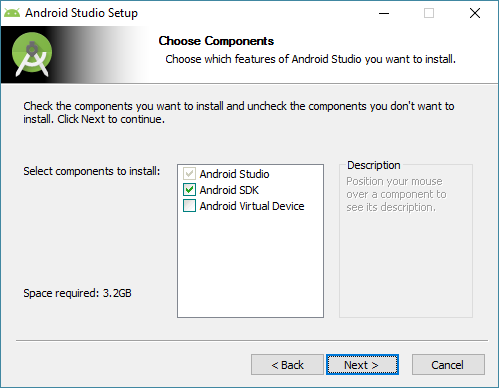
\includegraphics[width=0.65\textwidth]{android_studio_installer_01.png}
				\caption{Android Studio Setup > Komponenten ausw"ahlen. \label{studio_components}}
			\end{figure}
			%
			\newline
			Nach der Beendigung des Wizards erscheint noch der Dialog \glqq Complete Installation\grqq~, den wir noch durchlaufen m"ussen. Da wir von einer erstmaligen Installation von Android Studio ausgehen, w"ahlen wir die untere Option \glqq I do not have a previous version of Studio or I do not want to import my settings\grqq.
			\begin{figure}[h!]
				\centering
				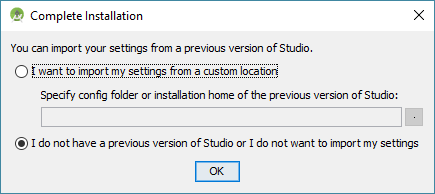
\includegraphics[width=0.55\textwidth]{android_studio_installer_02.png}
				\caption{Android Studio Dialog > Import Settings. \label{studio_import}}
			\end{figure}
			%
			\newpage
			Am SDK Components Setup Dialog angelangt, setzen wir H"akchen bei Android SDK, Android SDK Platform, API 23: Android 6.0 (Marschmallow). Die fehlenden Komponenten werden wir sp"ater manuell einrichten.
			\\ \newline
			\textbf{Wichtig!} Bei Android SDK Location den selben Pfad angeben, wie auch schon bei der Android SDK Installation Location.
			\begin{figure}[h!]
				\centering
				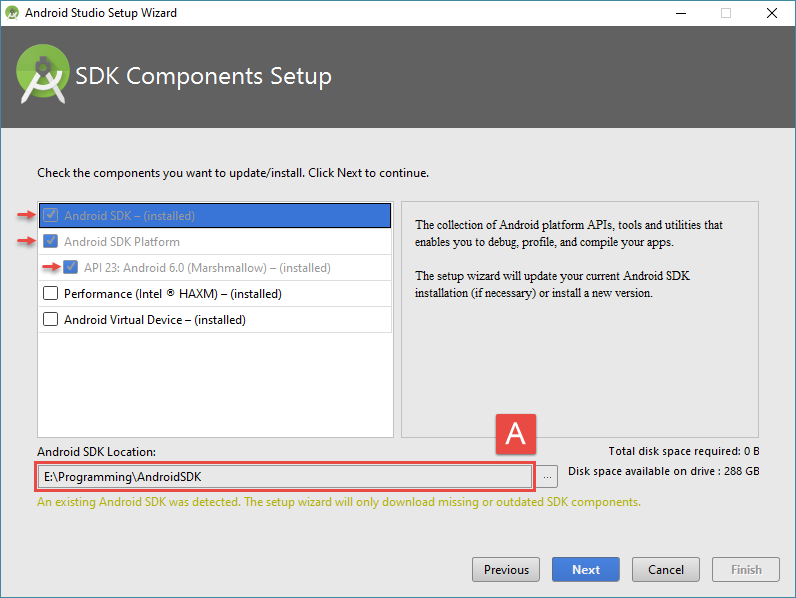
\includegraphics[width=0.8\textwidth]{android_studio_installer_03.png}
				\caption{Android Studio Dialog > SDK Components Setup. \label{studio_components_setup}}
			\end{figure}
			%
			\newpage
			Nach Abschluss der Installation w"ahlen wir im Willkommensbildschirm aus dem Quick Start-Men"u \glqq Configure\grqq~ und  klicken auf den vorletzten Men"ueintrag Check for Updates. Ist das Updaten abgeschlossen steht dem Entwickeln einer App nicht mehr viel im Weg.
			\begin{figure}[h!]
				\centering
				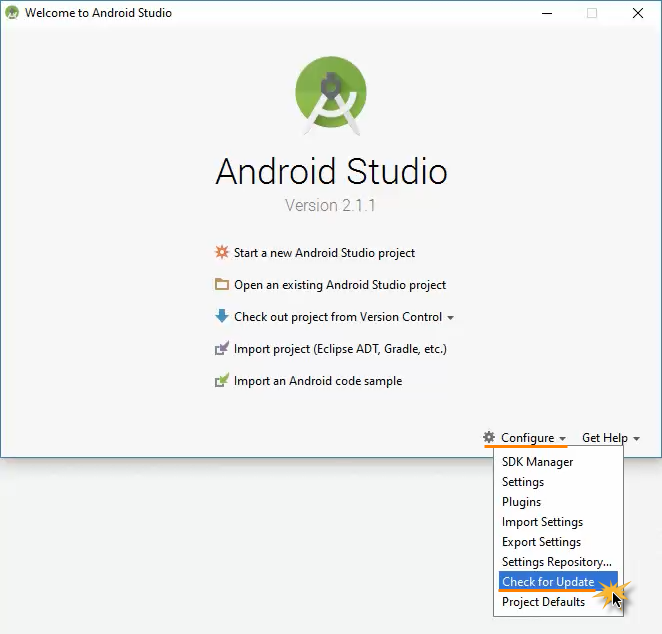
\includegraphics[width=0.8\textwidth]{android_studio_update.png}
				\caption{Android Studio: Updaten "uber Quick Start-Men"u. \label{studio_update}}
			\end{figure}
			%
			\newpage
			\subsection{Pr"ufung der installieren Packages}
			In der Bildserie folgenden werden alle Packages aufgef"uhrt die zur Entwicklung der App verwendet wurden. Es wird empfohlen diese zu installieren, um so maximale Kompatibilit"at zu gew"ahrleisten. Ihr "offnet den SDK Manager "uber das Quick Start-Men"u. Die jeweiligen Packages werden mit Hilfe des Standalone SDK Managers installiert (siehe Abb. \ref{studio_platforms})
			\begin{figure}[h!]
				\centering
				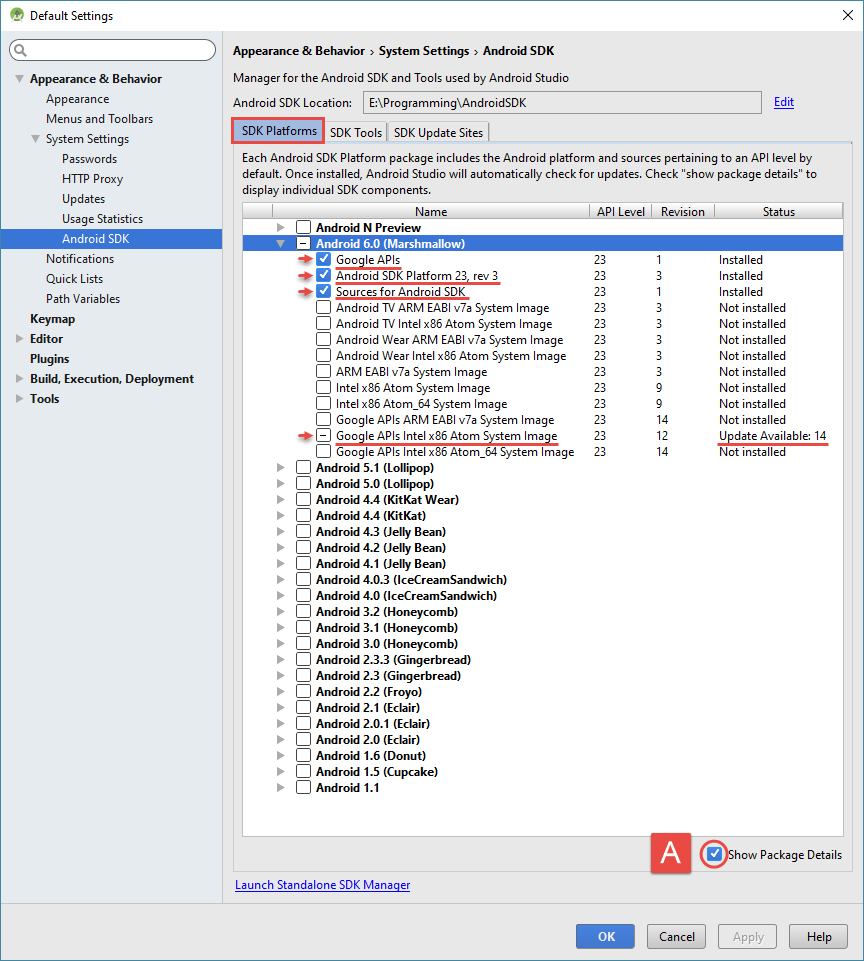
\includegraphics[width=0.9\textwidth]{android_studio_sdk_platforms.png}
				\caption{Android Studio: Installierte Packages der SDK Platforms.\label{studio_platforms}}
			\end{figure}
			\begin{figure}[h!]
				\centering
				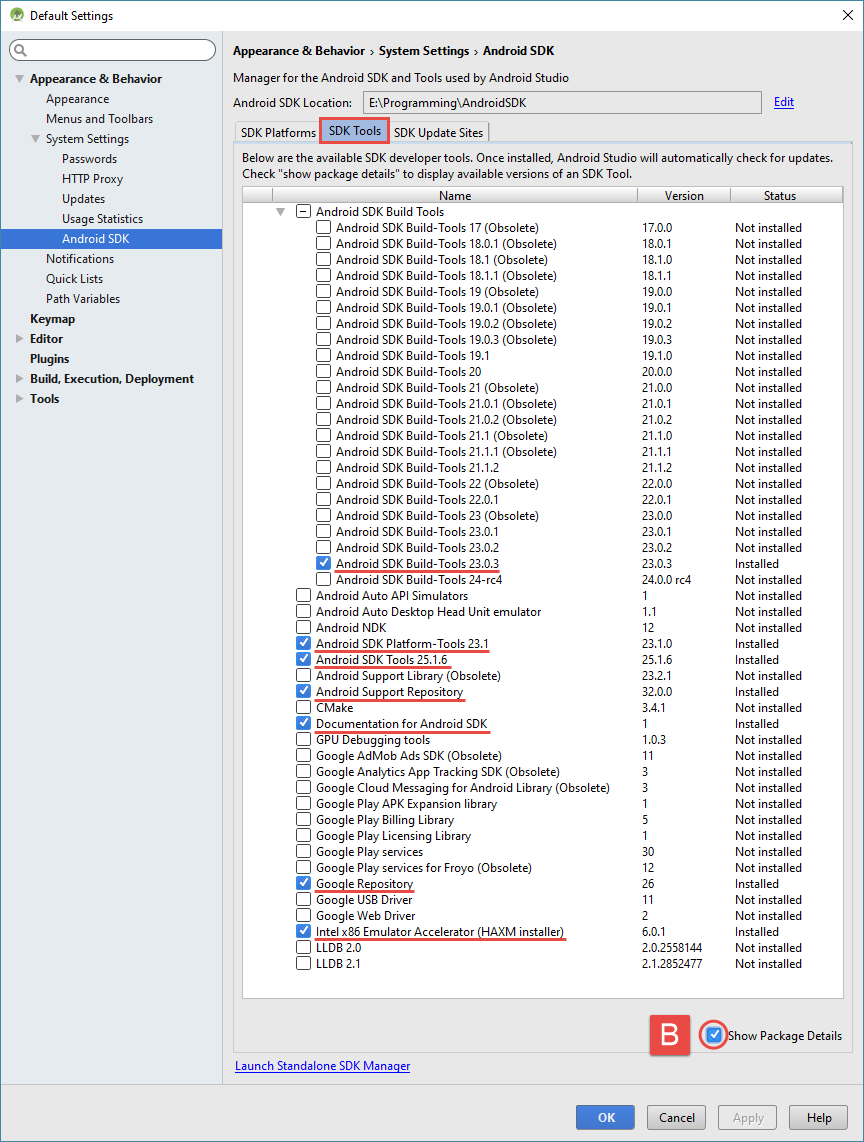
\includegraphics[width=\textwidth]{android_studio_sdk_tools.png}
				\caption{Android Studio: Installierte Packages der SDK Tools. \label{studio_tools}}
			\end{figure}
			 %
			 \newpage
			\subsection{Installation von Intel HAXM}
			Die Installationsdateien des INTEL HAXM (Hardware Accelerated Execution Manager) wurden bei der Installation von Android Studio bereits in das Verzeichnis des Android SDKs kopiert. Das Verzeichnis befindet sich unter folgendem Pfad:\\
			\path{...AndroidSDK\extras\intel\Hardware_Accelerated_Execution_Manager}
			\\ \newline
			Nachdem der HAXM-Installer gestartet wurde, "offnet sich der Willkommensbildschirm des Setup-Dialogs. Falls euer System die Systemvoraussetzungen nicht erf"ullt, wird die Installation automatisch abgebrochen. 
			\begin{figure}[h!]
				\centering
				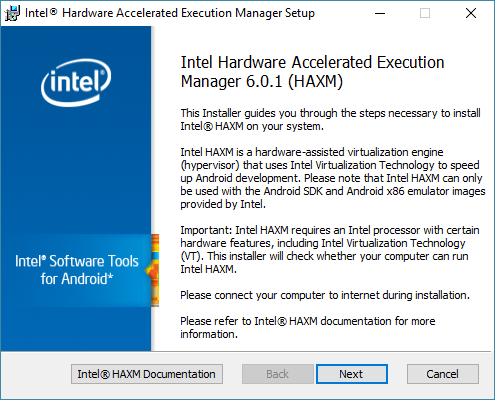
\includegraphics[width=0.8\textwidth]{android_studio_haxm_install_1.png}
				\caption{Intel HAXM Setup. \label{haxm_setup}}
			\end{figure}
			%
			\newline
			Im n"achsten Schritt wird nun nach einer Obergrenze f"ur den Arbeitsspeicher gefragt, die HAXM verwenden darf. Es kann die H"alfte des auf dem PC verf"ugbaren Arbeitsspeichers angegeben werden.
			\\ \newline
			\textbf{Achtung!} Dieser Wert sollte nicht zu hoch angesetzt werden, ansonsten k"onnten andere Programme langsamer ausgef"uhrt werden.
			%
			\newpage
			\begin{figure}[h!]
				\centering
				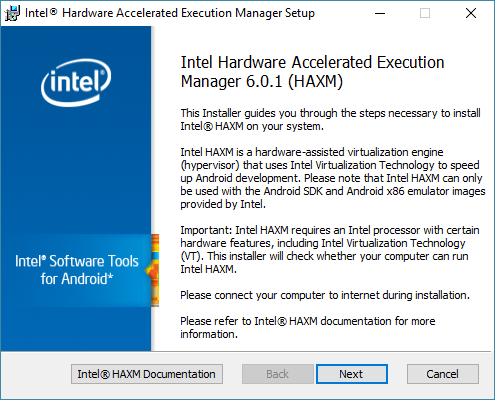
\includegraphics[width=0.8\textwidth]{android_studio_haxm_install_1.png}
				\caption{Arbeitsspeicherzuweisung an Intel HAXM. \label{haxm_storage}}
			\end{figure}
			%
			Nach abgeschlossener Installation gilt es noch zu Pr"ufen, ob Intel HAXM ordnungsgem"a"s auf dem System ausgef"uhrt wird. Hierf"ur starten wir die Kommandozeile als Administrator und verwenden folgenden Befehl: \textbf{sc query intelhaxm}.
			\begin{figure}[h!]
				\centering
				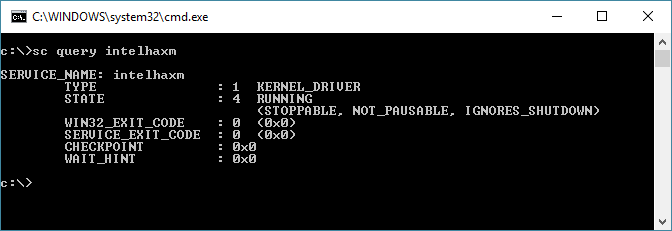
\includegraphics[width=0.8\textwidth]{android_studio_haxm_testen.png}
				\caption{Intel HAXM: Pr"ufung auf Systemausf"uhrung. \label{haxm_test}}
			\end{figure}
			%
			\newline
			Zeigt die Konsole \textbf{STATE: 4 running} oder "ahnliches an, wird Intel HAXM korrekt auf dem Rechner ausgef"uhrt.
		%
		\newpage
		\section{Android Virtual Device und Android Debugging Bridge}
			\subsection{AVD in Android Studio einrichten}
			Zur Ausf"uhrung einer App auf dem PC ben"otigen wir einen Android Emulator. Android Studio stellt uns f"ur diesen Zweck den Android Virtual Device Manager zur Verf"ugung. Die beiden M"oglichkeiten auf diesen zuzugreifen werden in den Abbildungen \ref{avd} und \ref{avd_tools} aufgef"uhrt.
			\begin{figure}[h!]
				\centering
				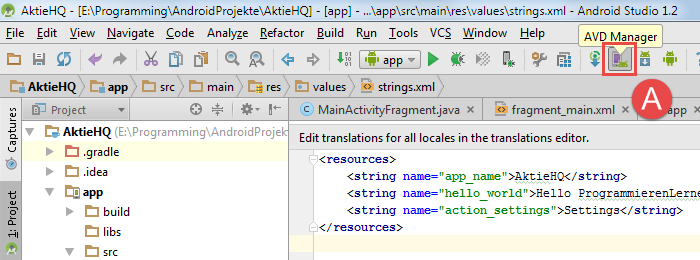
\includegraphics[width=0.8\textwidth]{android_studio_project_avd.png}
				\caption{Android Virtual Device Manager "uber AVD Manager-Icon. \label{avd}}
			\end{figure}
			\begin{figure}[h!]
				\centering
				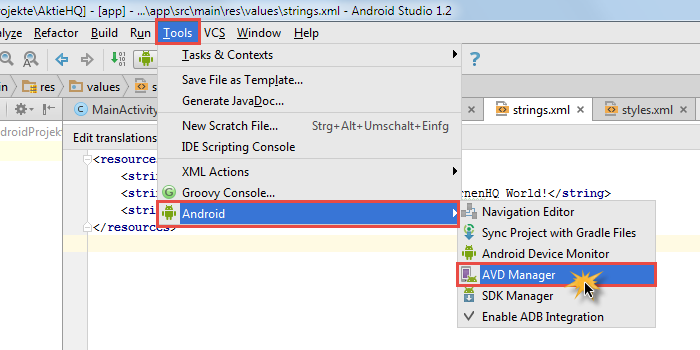
\includegraphics[width=0.8\textwidth]{android_studio_project_avd_manager.png}
				\caption{AVD Manager "uber Men"u. \label{avd_tools}}
			\end{figure}
			%
			\newline
			Nachdem der AVD Manager das erste Mal gestartet wurde, "offnet sich der Your Virtual Devices-Dialog des Managers. An dieser Stelle besteht die M"oglichkeit ein Android Virtual Device einzurichten.
			%
			\newpage
			\begin{figure}[h!]
				\centering
				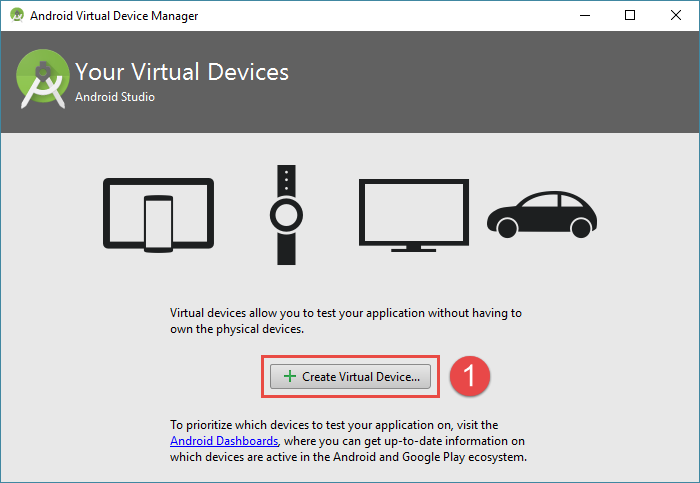
\includegraphics[width=0.8\textwidth]{android_studio_project_avd_1.png}
				\caption{Your Virtual Device Dialog. \label{avd_welcome}}
			\end{figure}
			%
			In den folgenden Bildschirmen lassen sich zu emulierendes Ger"at,System Image und Bildschirmorientierung bestimmen (Siehe Abb. \ref{avd_device} und \ref{avd_image}). Weitere Images k"onnen nach belieben zus"atzlich heruntergeladen werden.
			\begin{figure}[h!]
				\centering
				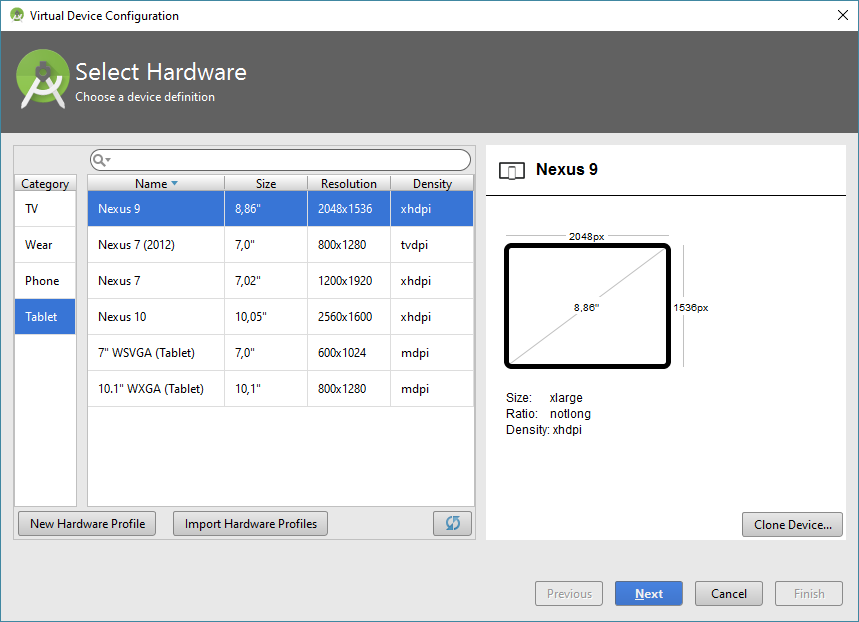
\includegraphics[width=0.8\textwidth]{android_studio_project_avd_2.png}
				\caption{AVD Device Selection. \label{avd_device}}
			\end{figure}
			%
			\newpage
			\begin{figure}[h!]
				\centering
				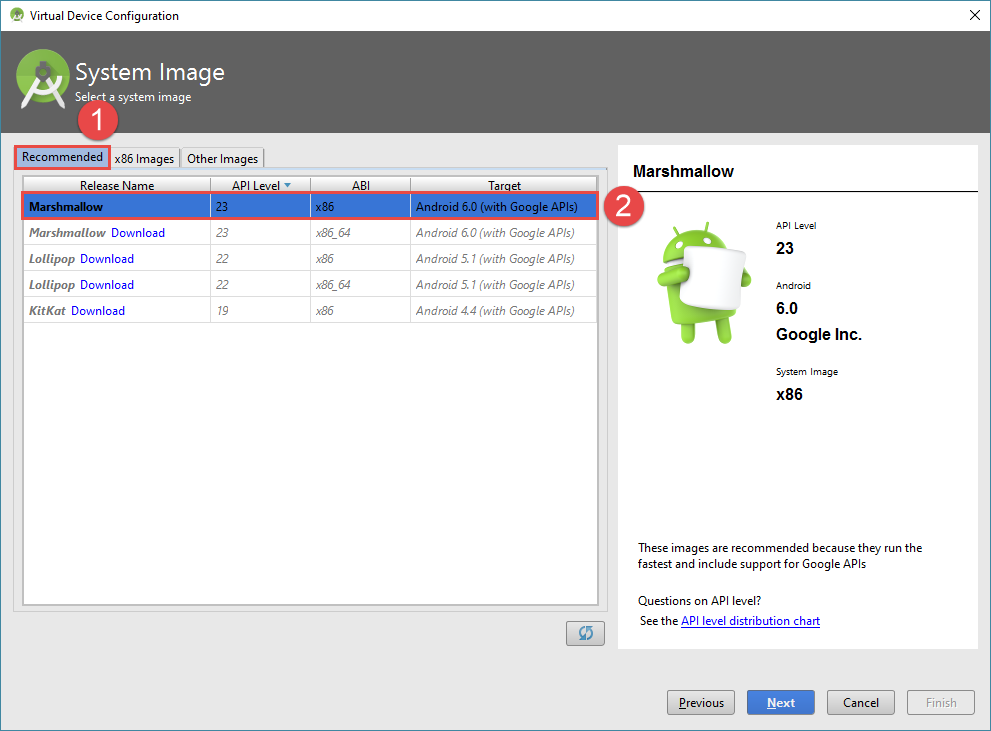
\includegraphics[width=0.8\textwidth]{android_studio_project_avd_3.png}
				\caption{AVD System Image Selection. \label{avd_image}}
			\end{figure}
			%
			Anschlie�end l"asst sich das emulierte Ger"at entweder "uber den AVD Manager oder das Run-Icon starten. Dieser Vorgang ben"otigt unter Umst"anden einige Minuten.
			\begin{figure}[h!]
				\centering
				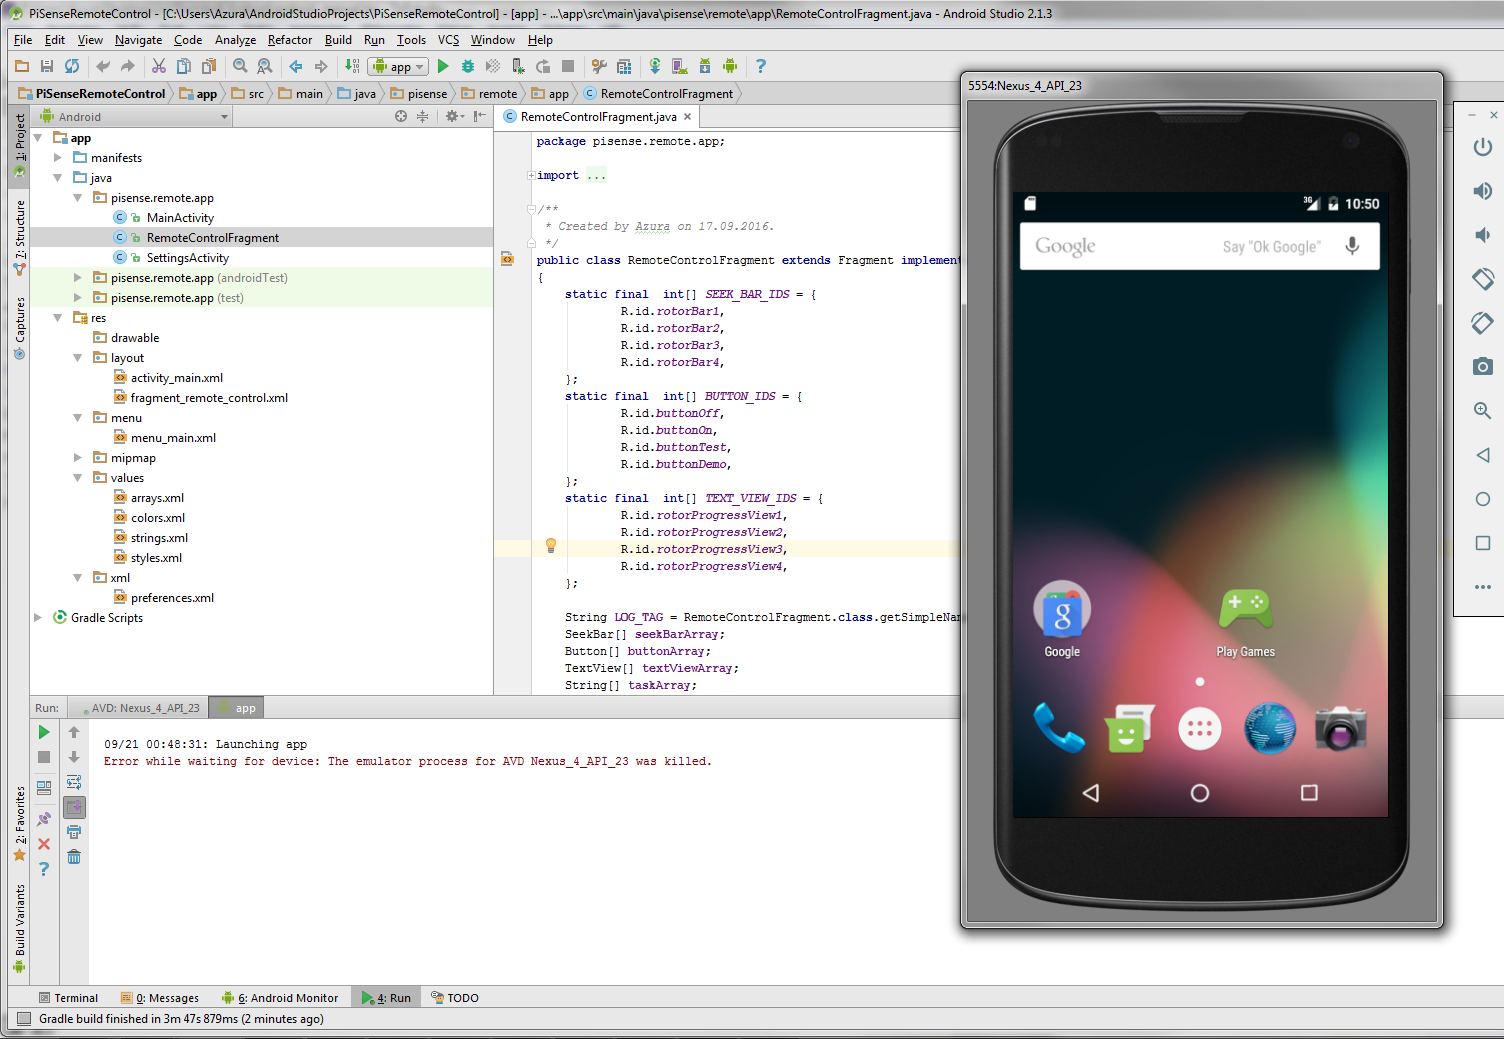
\includegraphics[width=0.8\textwidth]{emulated_device.png}
				\caption{Emuliertes Nexus 4 mit Android 6.0. \label{avd_emulate}}
			\end{figure}
			%
			\newpage
			\subsection{Einrichten der Android Debugging Bridge (ADB)}
			Das Aufbauen einer Android Debugging Bridge, ben"otigt zun"achst das Aktivieren der Entwicklereinstellungen auf dem Smartphone (Siehe Abb. \ref{avd_dev}). Diese sind auf Ger"aten mit Android 4.2 oder neuer standardm"a"sig versteckt.
			\begin{figure}[h!]
				\centering
				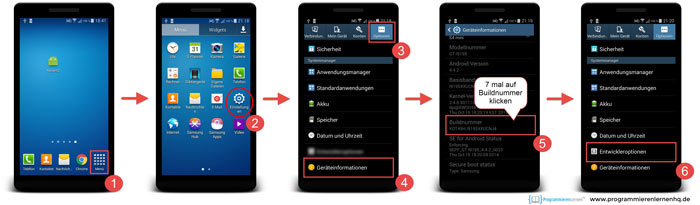
\includegraphics[width=0.9\textwidth]{android_entwickleroptionen_aktivieren_anleitung_1_tn.png}
				\caption{Android Entwickleroptionen aktivieren. \label{avd_dev}}
			\end{figure}
			%
			\newline
			Nachdem die Android Entwickleroptionen aktiviert wurden. M"ussen zwingend bei \glqq wach bleiben\grqq~und \glqq USB-Debugging\grqq~H"akchen gesetzt werden (Siehe Abb. \ref{avd_debug}). USB-Debugging erlaubt dem angeschlossenen Rechner die Kommunikation mit dem Android Ger"at.
			\begin{figure}[h!]
				\centering
				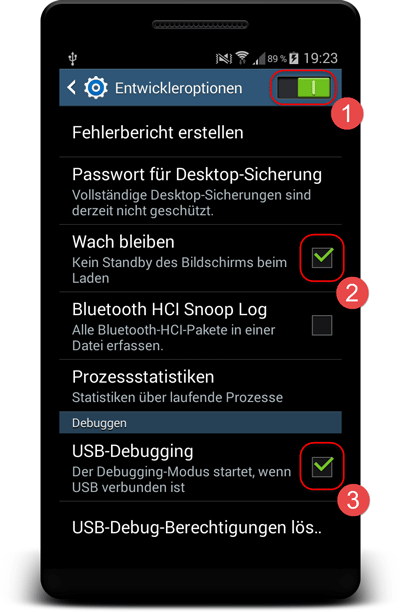
\includegraphics[width=0.4\textwidth]{android_usb_debugging_aktivieren_tn.png}
				\caption{USB-Debugging und wach bleiben aktivieren. \label{avd_debug}}
			\end{figure}
			%
			\newpage
			Damit eine Verbindung des PCs mit dem Android Ger"at m"oglich ist, muss der passende USB Treiber f"ur das Smartphone oder Tablet auf unserem System installiert werden:
			\begin{itemize}
				\item Android Developer Phones, wie Nexus One oder Nexus S, ben"otigen die Google USB Treiber: \url{http://developer.android.com/sdk/win-usb.html}
				\item Einer Liste anderer Hersteller mit Treiber URL findet man hier:\\
				\url{http://developer.android.com/tools/extras/oem-usb.html#Drivers}
			\end{itemize}
			 %
			 Das Ansteuern des Android Ger"ates erfolgt "uber die Konsole im Verzeichnis \path{..\AndroidSDK\platform-tools} oder das Terminal in Android Studio. Mit dem Befehl \textbf{adb devices} lassen sich angeschlossene Ger"ate anzeigen.
			 \begin{figure}[h!]
			 	\centering
			 	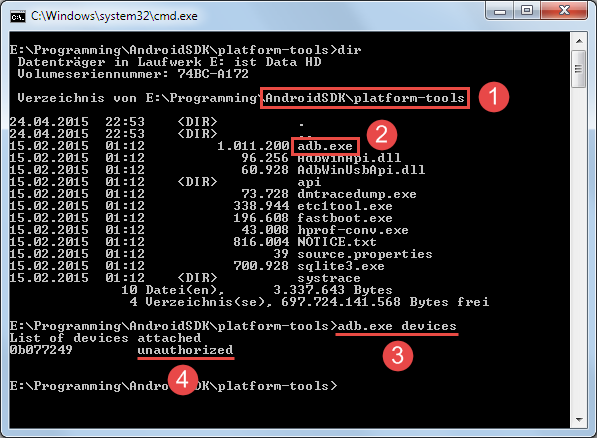
\includegraphics[width=0.8\textwidth]{android_adb_devices_unauthorized1.png}
			 	\caption{Angeschlossene Ger"ate mit Hilfe der ADB anzeigen lassen. \label{adb_devices}}
			 \end{figure}
			 %
			 \newline
			 Das Ger"at ist zu diesem Zeitpunkt noch nicht autorisiert und eine Verbindung unm"oglich. Hierbei handelt es sich um einen Schutzmechanismus aller Android Ger"ate ab Android 4.2.2, um vor unberechtigten Zugriff zu sch"utzen. Die Autorisierung erfolgt "uber das Android Ger"at, in einem Dialog bittet es um einen RSA-Handshake.
			 %
			 \newpage
			 \begin{figure}[h!]
			 	\centering
			 	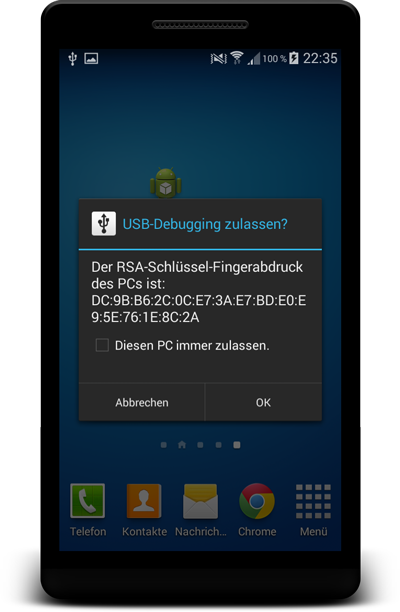
\includegraphics[width=0.4\textwidth]{RSA_Handshake_tn.png}
			 	\caption{RSA-Schl"ussel-Fingerabdruck. \label{rsa}}
			 \end{figure}
			%
			Um den oben beschriebenen USB-Debugging Dialog anzeigen zu lassen und eine Verbindung zum Android Ger"at anzufordern, verwenden wir folgende ADB-Befehle in der Konsole (die Dateiendung .exe ist nicht zwingend erforderlich):
			\begin{itemize}
				\item Beenden des ADB Servers mit: \textbf{adb.exe kill-server} 
				\item Starten des ADB Servers mit: \textbf{adb.exe start-server}
			\end{itemize}
			%
			\textbf{Achtung!} Sicher stellen, dass der Bildschirm des Android Ger"ates entriegelt ist!
			\begin{figure}[h!]
				\centering
				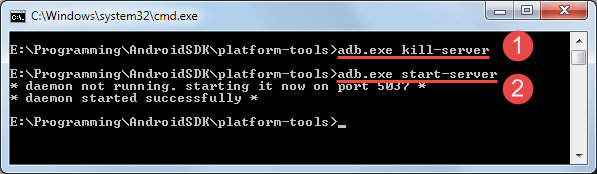
\includegraphics[width=0.8\textwidth]{android_adb_server1.png}
				\caption{ADB Server Neustart.\label{adb_kill}}
			\end{figure}
			%
			\newpage
			Nach erfolgreicher Ausf"uhrung, sollte der Befehl \textbf{adb devices} das Android Ger"at als device f"uhren. Eine Installation der App auf dem Zielger"at, ist nun mit Hilfe des Run-Icons in Android Studio m"oglich.
			\begin{figure}[h!]
				\centering
				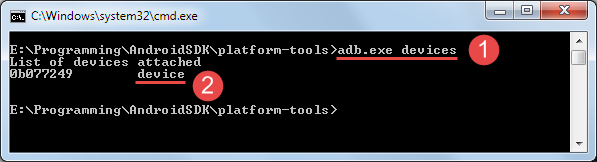
\includegraphics[width=0.8\textwidth]{android_adb_device1.png}
				\caption{Android Ger"at erfolgreich als device gelistet.\label{adb_done}}
			\end{figure}
		%
		\section{Git}
			\subsection{Installation von Git}
			Die Verwendung von Git auf Windows 7 erfordert zun"achst die Installation einer Git Shell, wie beispielsweise Git BASH. 
			\begin{itemize}
				\item \url{https://git-for-windows.github.io/}
			\end{itemize}
			%
			Mit Hilfe der Help Dokumentation im Atreus lassen sich schnell Probleme, wie die Initialisierung des global user.names, der global user.email und das Generieren eines SSH-Keys bewerkstelligen (Siehe Abb \ref{git_help}).
			\begin{figure}[h!]
				\centering
				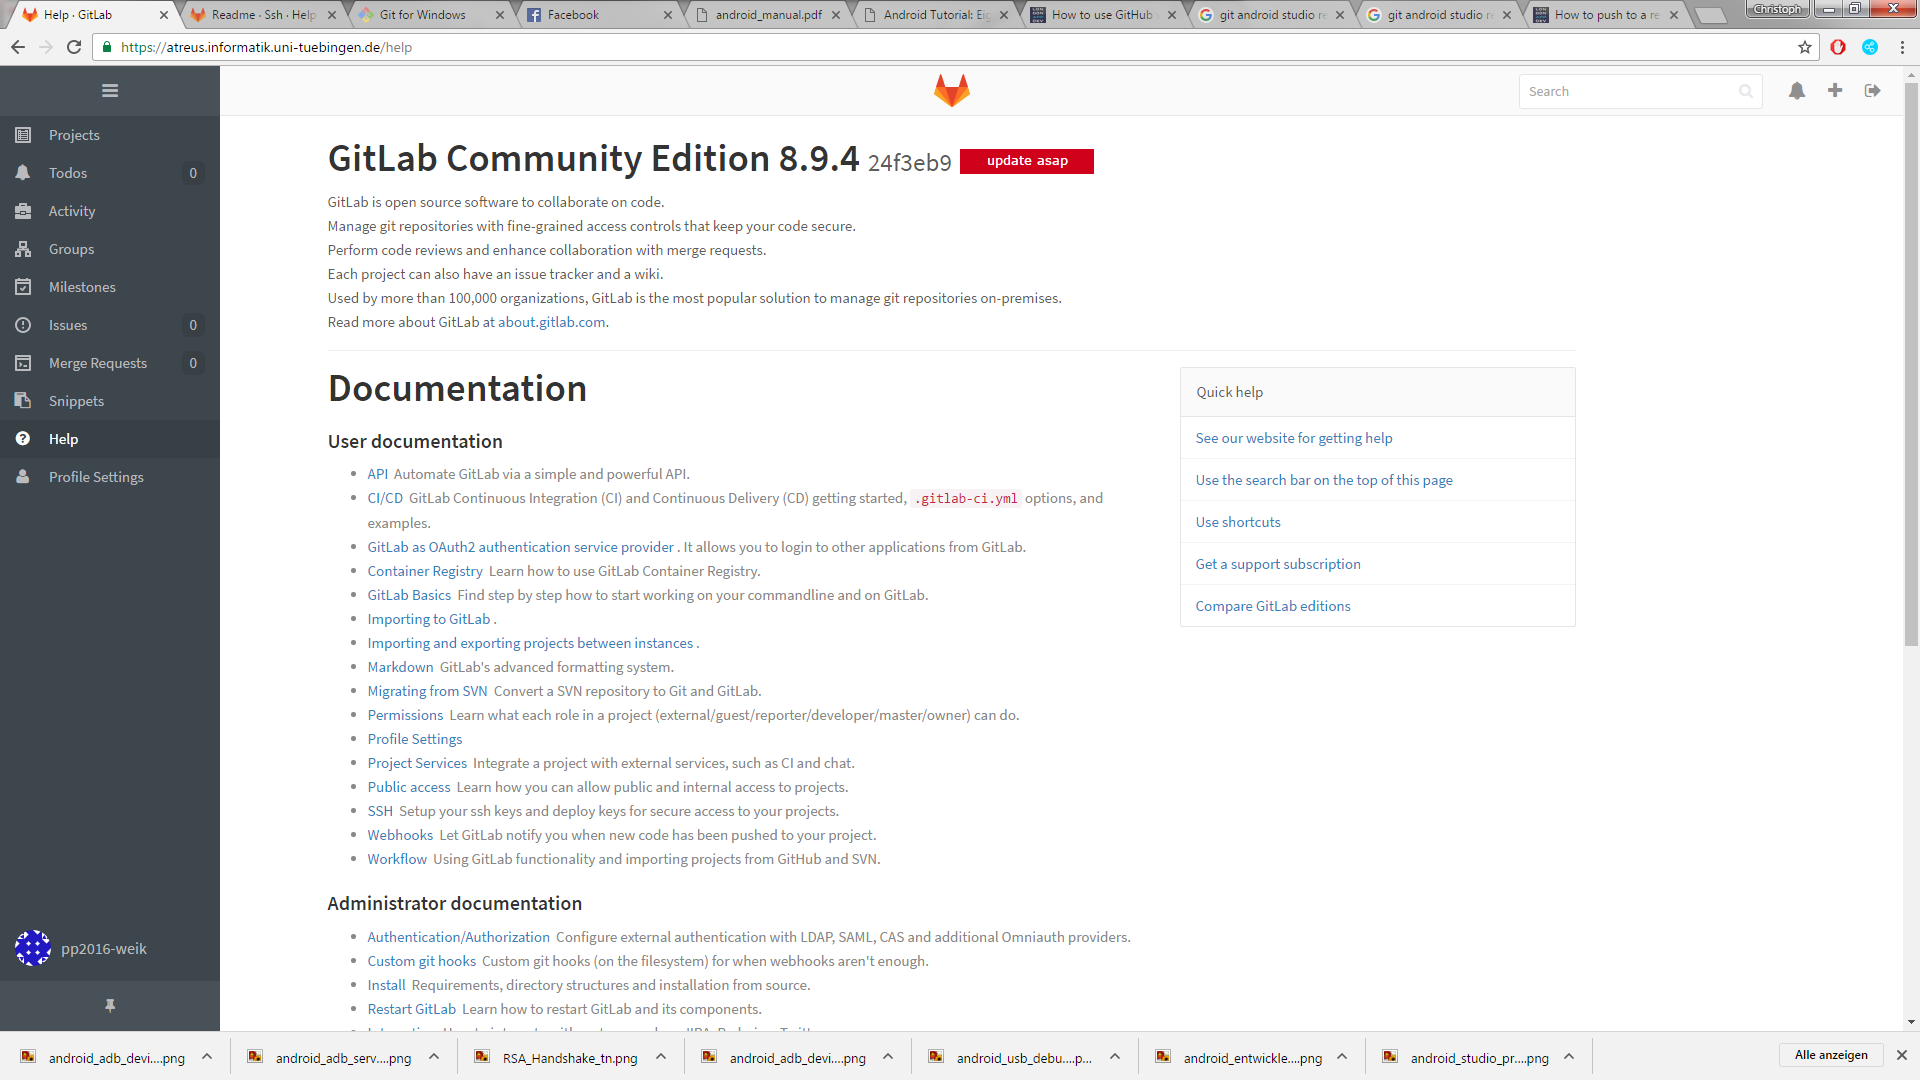
\includegraphics[width=0.95\textwidth]{git_help.png}
				\caption{Help Dokumentation in Atreus.\label{git_help}}
			\end{figure}
			%
			\newpage
			\subsection{Git in Android Studio}
			Im Folgenden handelt es sich um eine Step-by-Step Anleitung zur Einrichtung von Git als Version Control in Android Studio. Zu Beginn navigieren wir zu den Git Version Control Settings "uber File > Settings > Version Control > Git (Siehe Abb. \ref{git_set1}). In Windows 7 ist default Pfad der git.exe \path{C:\Program Files\Git\cmd\git.exe} diesen tragen wir in \glqq Path to executable\grqq~ein. Ein erfolgreicher Test sollte eine R"uckmeldung wie in Abbildung \ref{git_set2} geben.
			\\ \newline
			\textbf{Wichtig!} SSH-executable auf Built-in lassen.
			\begin{figure}[h!]
				\centering
				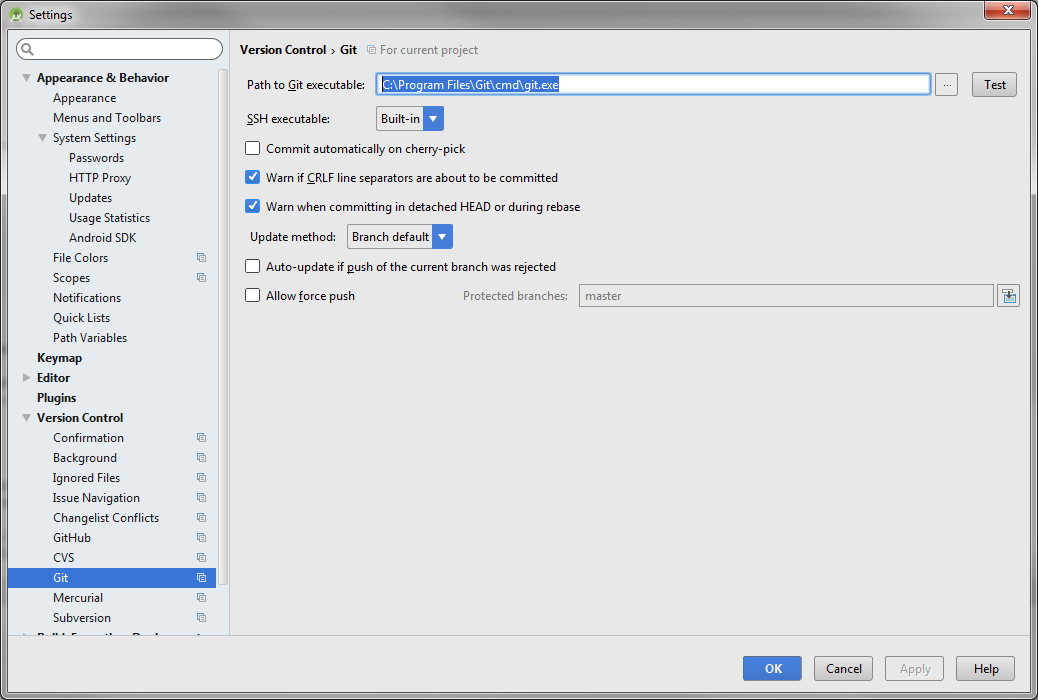
\includegraphics[width=0.8\textwidth]{git_settings1.png}
				\caption{Version Control Settings.\label{git_set1}}
			\end{figure}
			\begin{figure}[h!]
				\centering
				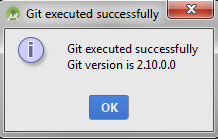
\includegraphics[width=0.3\textwidth]{git_settings2.png}
				\caption{Git erfolgreich ausgef"uhrt.\label{git_set2}}
			\end{figure}
			%
			\newpage
			Anschlie"send schlie"sen wir das aktuelle Fenster wieder und erstellen mit den n"achsten Schritten ein lokales Git Repository in Android Studio. Dazu navigieren wir "uber VCS > Import into Version Control > Create Git Repository (Siehe Abb. )
			\begin{figure}[h!]
				\centering
				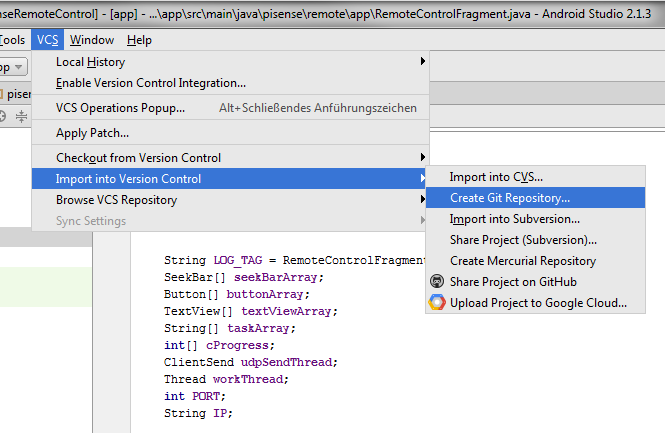
\includegraphics[width=0.7\textwidth]{git_local_repo.png}
				\caption{Men"u Navigation \glqq Create Git Repository\grqq\label{git_repo1}}
			\end{figure}
			%
			\newline
			Als n"achstes designieren wir das Verzeichnis, welches von Git initialisiert werden soll. Hier bietet es sich an das Projektverzeichnis zu w"ahlen. Im Folgenden "offnen wir den Pfad unseres Projektverzeichnisses und starten "uber das Rechtsklickmen"u Git BASH (Siehe Abb. \ref{git_bash})
			\begin{figure}[h!]
				\centering
				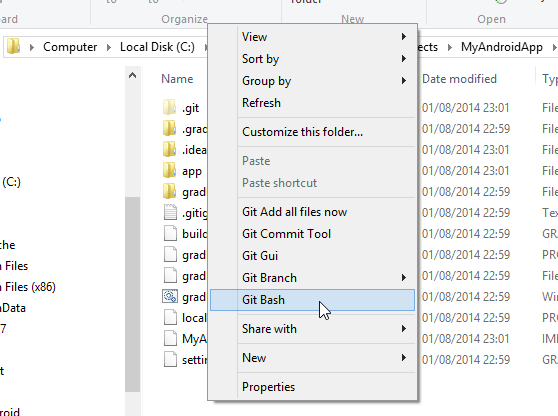
\includegraphics[width=0.7\textwidth]{bash.png}
				\caption{Starten von Git BASH im Projektverzeichnis\label{git_bash}}
			\end{figure}
			%
			\newpage
			Im Git BASH angekommen m"ochten wir das gew"unschte Remote Repository hinzuf"ugen. Dies geschieht "uber den Befehl:\\
			\textbf{git remote add origin \path{ssh://[user]@[server_address]/[git_repo_url]}}\\
			In unserem Fall w"are die gew"unschte Adresse (aus Atreus):\\ \path{git@atreus.informatik.uni-tuebingen.de:Programmierprojekt2016/QuadrocopterAndroid.git}.
			\begin{figure}[h!]
				\centering
				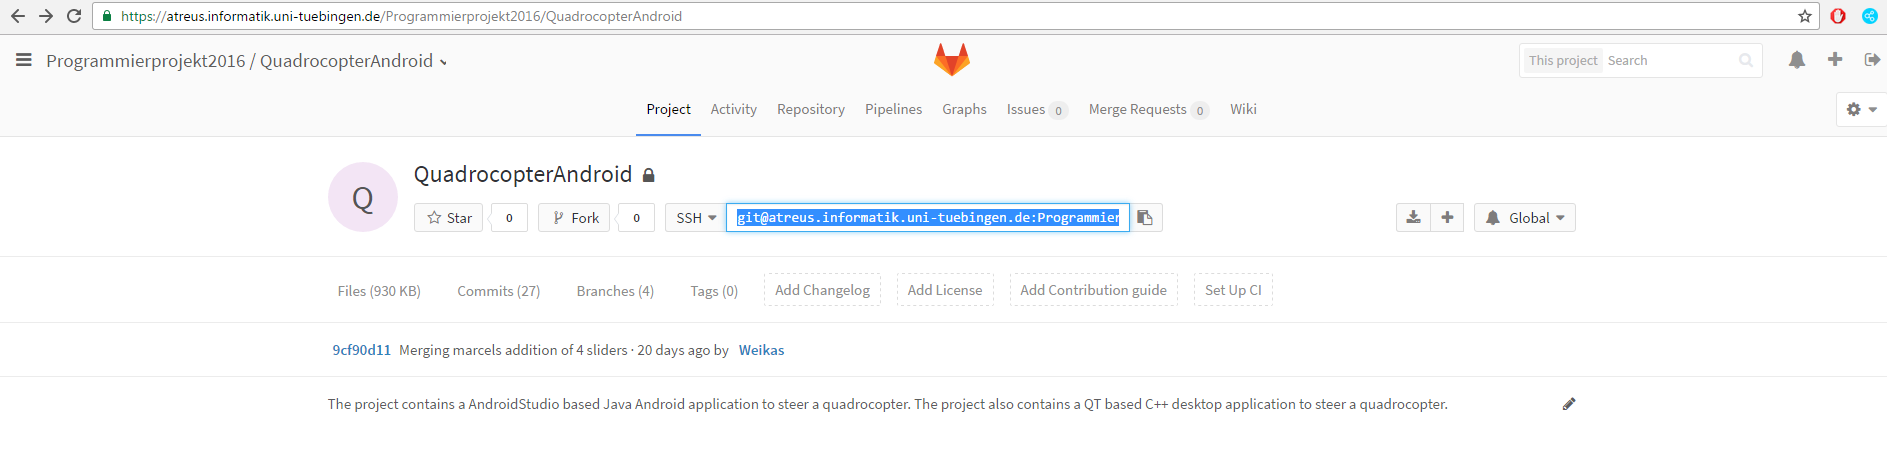
\includegraphics[width=0.8\textwidth]{git_origin.png}
				\caption{SSH Adresse des Repositories in Atreus.\label{git_origin}}
			\end{figure}
			\begin{figure}[h!]
				\centering
				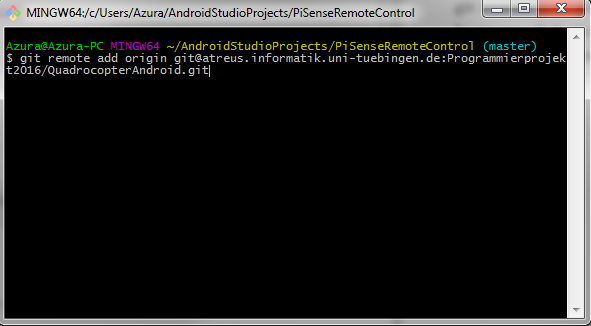
\includegraphics[width=0.65\textwidth]{git_origin_cmd.png}
				\caption{Hinzuf"ugen eines Remote Repositories in Git BASH.\label{git_cmd}}
			\end{figure}
			%
			\newline
			Um nun erfolgreich an der bereits gestellten App weiter programmieren zu k"onnen muss das Projekt erst von Git geklont werden. Dies ist m"oglich "uber VCS > Checkout from Version Control > Git. Im folgenden Fenster tragen wir die Ziel URL ein, sowie den Namen des Branches den wir klonen wollen (Siehe Abb. \ref{git_clone}).
			\begin{figure}[h!]
				\centering
				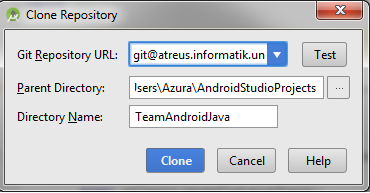
\includegraphics[width=0.45\textwidth]{git_clone.png}
				\caption{Ein Projekt mit Android Studio von Git klonen.\label{git_clone}}
			\end{figure}
			%
			\newpage
			Der Ablauf eines erfolgreichen Commits ist wie folgt: Hinzuf"ugen der Daten zum Git Reository > Committen des Verzeichnisses und hinterlassen einer Commit Nachricht > Pushen aller "Anderungen auf das Remote Repository und angegebenen Branch.
			\begin{figure}[h!]
				\begin{subfigure}[b]{0.5\textwidth}
					\centering
					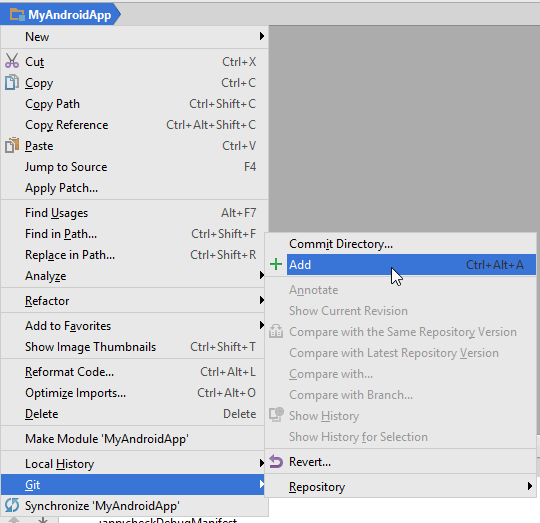
\includegraphics[width=0.8\textwidth]{add1.png}
					\subcaption{Add}
				\end{subfigure}
				\begin{subfigure}[b]{0.5\textwidth}
					\centering
					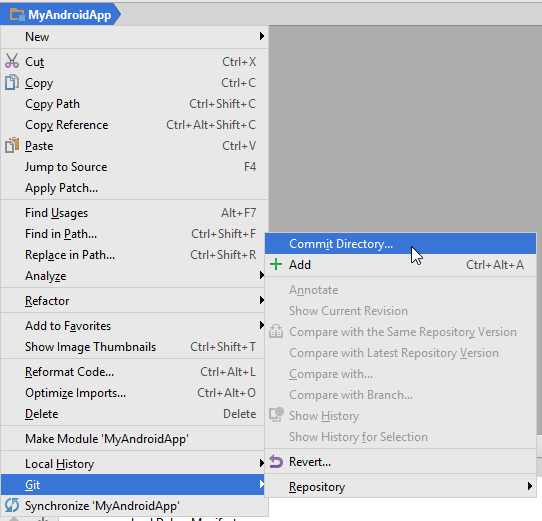
\includegraphics[width=0.8\textwidth]{commit1.png}
					\subcaption{Commit}
				\end{subfigure}
				\begin{subfigure}[h!]{1\textwidth}
					\centering
					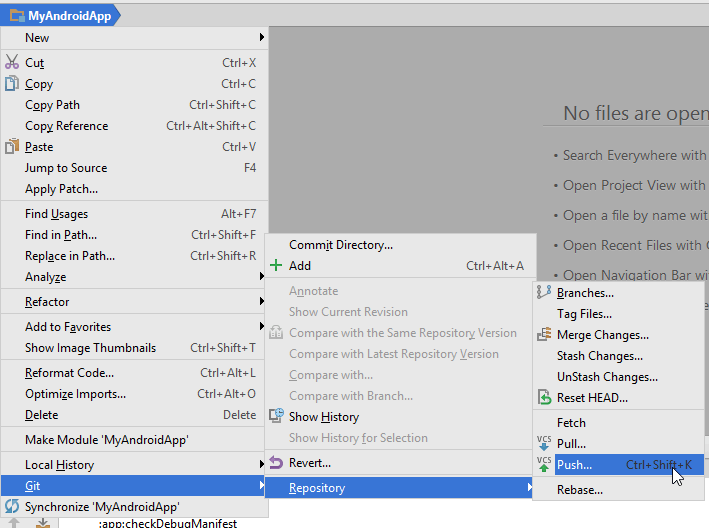
\includegraphics[width=0.5\textwidth]{push1.png}
					\subcaption{Push.\label{push1}}
				\end{subfigure}
				\caption{Men"u Navigation zu Add, Commit und Push.\label{add_com}}
			\end{figure}
	%
	\chapter{Android Applikation}
		\section{Einleitung}
			\subsection{Ressourcen}
			Effektives Ressourcen-Management in Android Studio gestaltet die Entwicklung einer App sehr unkompliziert und "ubersichtlich. S"amtliche Informationen "uber GUI Elemente, Strings, Men"ubausteine oder auch Pr"aferenzen werden in XML Dokumente leicht zug"anglich abgelegt und kommen der Lesbarkeit des Codes zugute.
			\begin{figure}[h!]
				\centering
				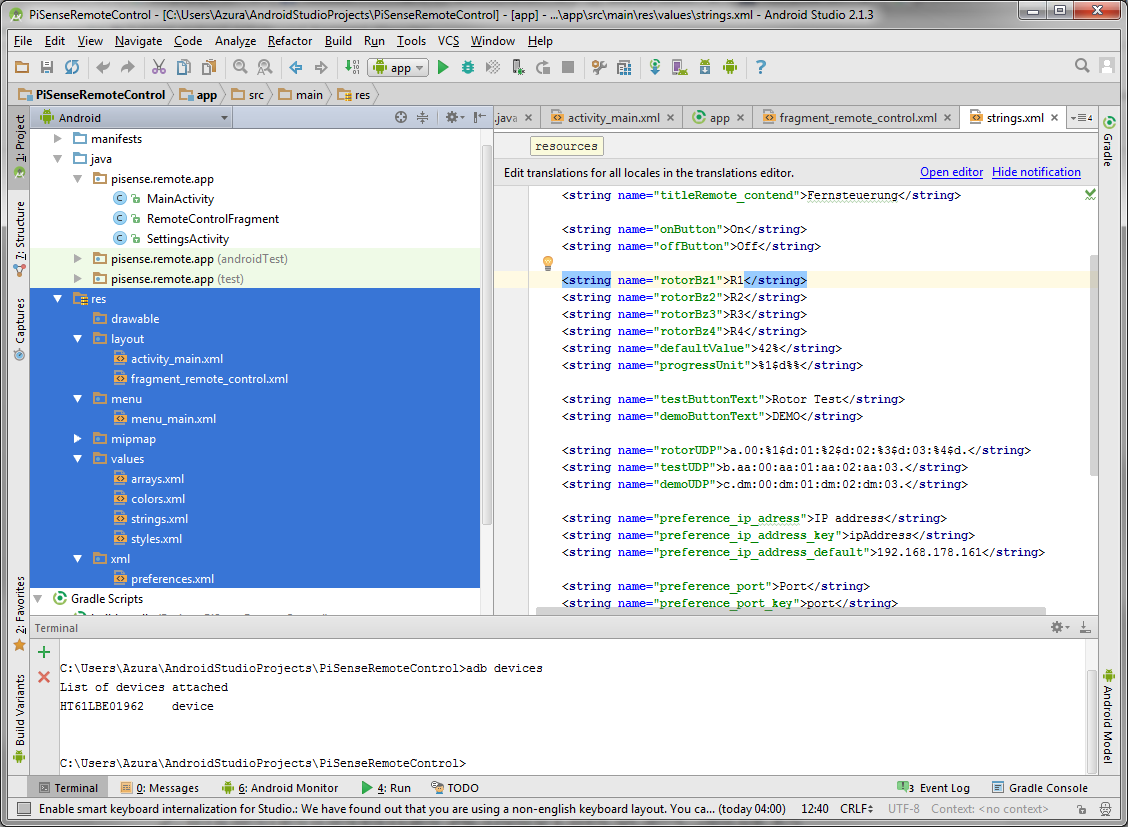
\includegraphics[width=0.8\textwidth]{resource.png}
				\caption{Beispielhafte Darstellung der String Ressource unserer App.\label{resource}}
			\end{figure}
			%
			\newpage
			\subsection{Activity}
			Eine Activity ist ein Bestandteil einer Anwendung, die einen Bildschirm zur Verf"ugung stellt, mit dem der Benutzer interagieren kann. Im Regelfall besteht eine App aus mehreren Activities die lose miteinander verbunden sind. Jede Activity besitzt die F"ahigkeit eine andere Activity zu starten, dabei wird die Aktuelle gestoppt und die Gestartete r"uckt in den Fokus. Der Zustand der gestoppten Activity bleibt jedoch im Android System erhalten. Dies ist der Moment wenn sogenannte Lifecyle-Callbacks in Kraft treten. Diese informieren die Activity "uber eintretende Zustands"anderungen und geben die Gelegenheit bestimmte, notwendige Arbeit zu verrichten, bevor diese Zustands"anderung eintritt.
			\begin{figure}[h!]
				\centering
				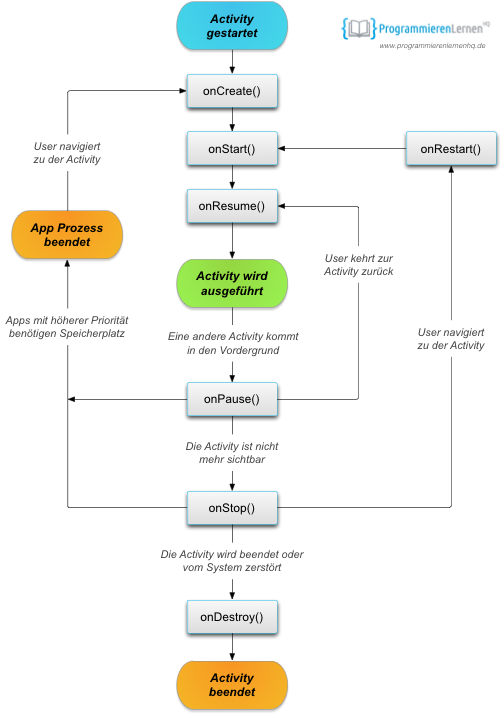
\includegraphics[width=0.65\textwidth]{android_activity_lifecycle_tn_.png}
				\caption{Callback-Methoden des Activity Lifecyle in Android.\label{activity_lc}}
			\end{figure}
			%
			\newpage
			\textbf{Achtung!} Implementiert man eine dieser Lifecycle-Methoden, ist es zwingen notwendig zuerst die Implementierung der Basisklasse aufzurufen.
			\begin{verbatim}
			protected void onPause() {
			super.onPause(); // Aufrufen der Implementierung der Superklasse
			// Hier folgt der eigene Code
			}
			\end{verbatim}
			%
			\subsection{Fragment}
			Bei Fragmenten handelt es sich um Modulare Bereiche einer Activity. Diese verf"ugen "uber ihre eigenen Lifecycle und Callback-Methoden. Der "ubergeordnete Activity-Lifecycle beeinflusst den Fragment-Lifecycle direkt. Das hei�t, pausiert bzw. wird die Activity zerst"ort, dann tut dies auch das zugeh"orige Fragment. Eine Activity kann "uber mehrere Fragmente verf"ugen und diese k"onnen auch in mehreren Activities wiederverwendet werden. Fragmente m"ussen nicht zwingend Teil des Activity Layouts sein, sie k"onnen auch als unsichtbare Arbeiter eingegliedert werden.
			\begin{figure}[h!]
				\centering
				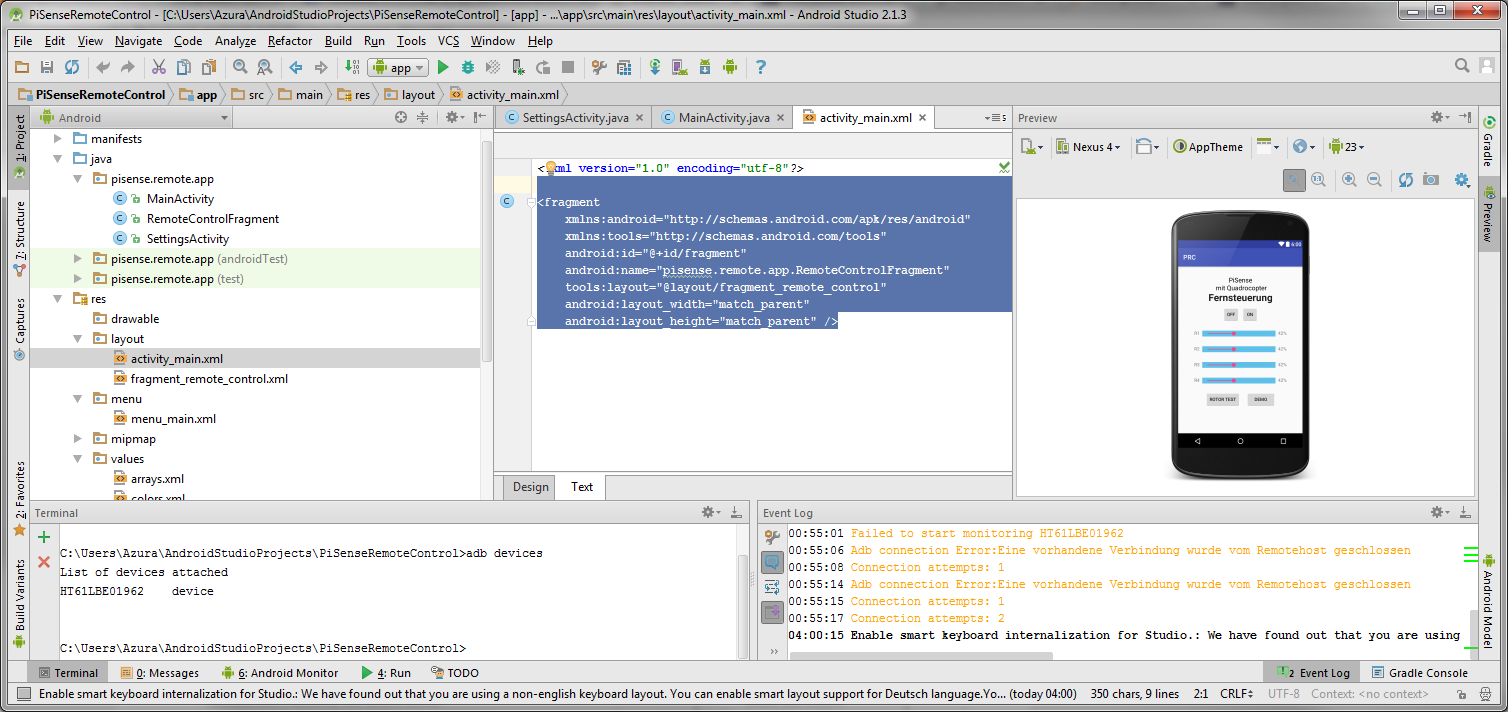
\includegraphics[width=0.9\textwidth]{activity_style.png}
				\caption{Activity wird vollst"andig mit Fragment Layout ausgef"ullt. \label{ac_lay}}
			\end{figure}
			\newpage
			\begin{figure}[h!]
				\centering
				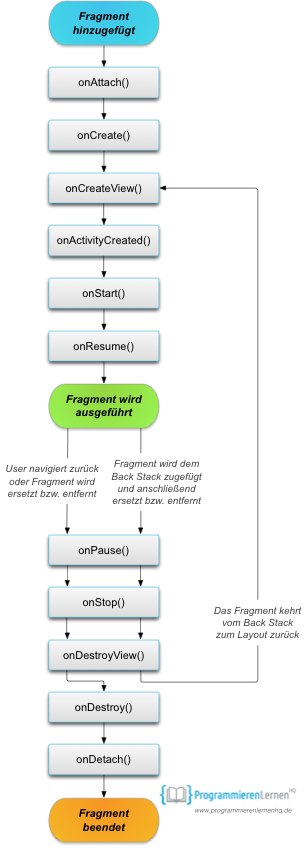
\includegraphics[height=1.2\textwidth]{android_fragment_lifecycle_tn.png}
				\caption{Callback-Methoden des Fragment Lifecyle in Android.\label{fragment_lc}}
			\end{figure}
		%
		\newpage
		\section{Layout}
		Das Layout der App wurde vollst"andig mithilfe des GUI Editors von Android Studio erstellt. Nach Erstellung der notwendigen layout.xml erzeugt dieser automatisch das passende XML Gegenst"uck zum jeweiligen GUI Element. Die in der App verwendete Oberfl"ache gestaltet sich wenig komplex, hierbei handelt es sich mehrere ineinander geschachtelte horizontale und vertikale Layouts. Eingef"ugt wurden jeweils die gew"unschten Buttons, Textfelder und Seekbars.
		\\ \newline
		\textbf{Achtung!} Editiert wird indem Layouts und GUI-Elemente in den Component Tree rechts oben gezogen werden.
		\begin{figure}[h!]
		\centering
		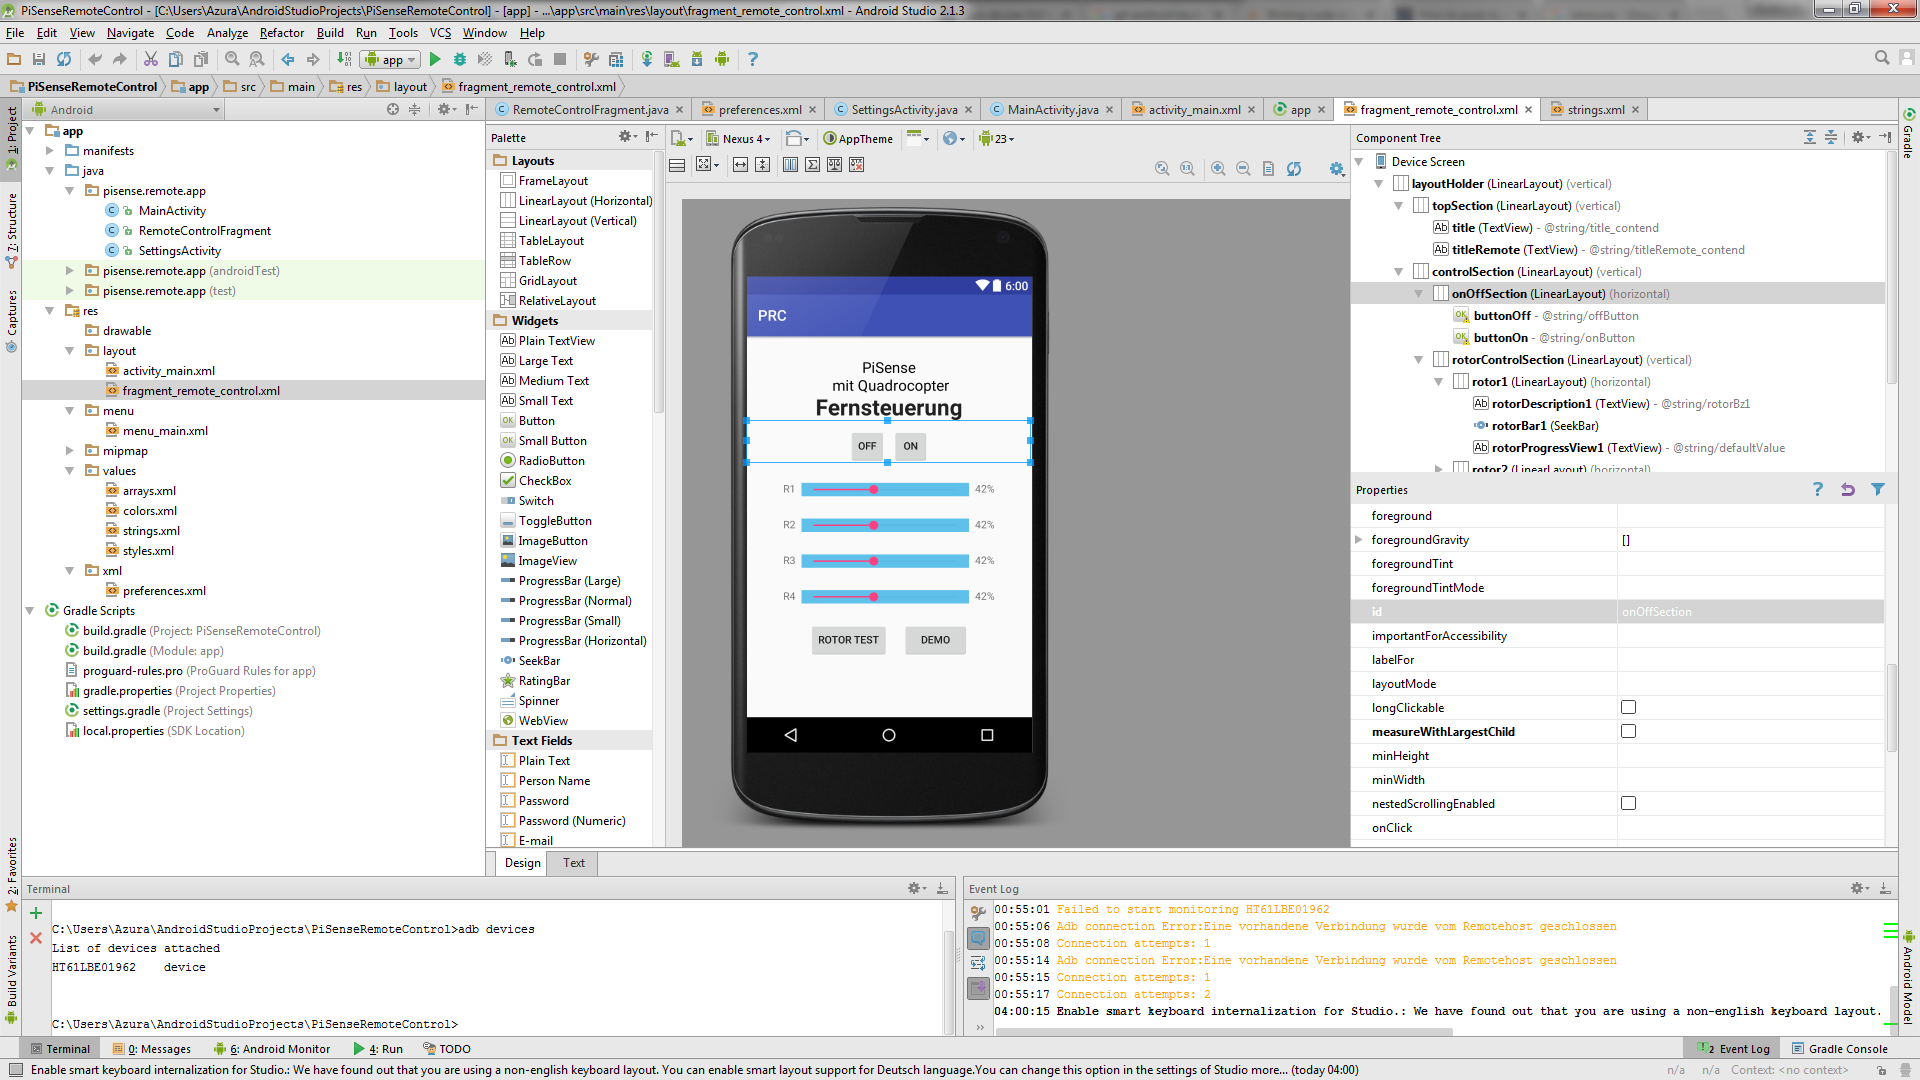
\includegraphics[width=\textwidth]{layout.png}
		\caption{GUI Editor in Android Studio.\label{layout}}
		\end{figure}
		%
		\newpage
		Eigenschaften der jeweiligen Elemente wird durch das Properties Men"u unten rechts beeinflusst. Hier lassen sich Ausrichtung (gravity), Abst"ande (padding, margin...), Farbe und vieles mehr bestimmen. Eines der wichtigsten Attribute ist jedoch die \textbf{id} hiermit lassen sich Layout-Elemente im Editor benennen und im Code auf deren Layout zugreifen. Buttons, TextViews und SeekBars werden mithilfe der ID Objekte auf denen dann Arbeit verrichtet werden kann. F"ur Buttons und SeekBars war es des Weiteren notwendig Listener zu implementieren, die auf Zustands"anderungen reagieren k"onnen (Siehe Abb. \ref{buttons}).
		\begin{figure}[h!]
			\centering
			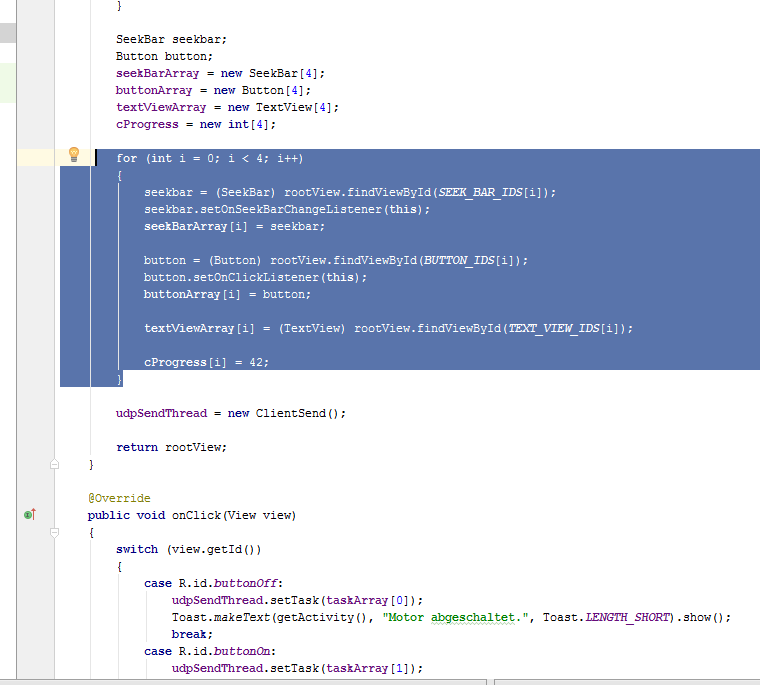
\includegraphics[width=0.8\textwidth]{buttons.png}
			\caption{For-Schleife zur Bindung von Listenern an View-Objekte.\label{buttons}}
		\end{figure}
		%
		\newpage
		\section{Funktion}
		Die angedachte Funktion der Applikation ist es Befehlsketten auf Aktivierung der jeweiligen Buttons per UDP an den Raspberry Pi zu schicken. Dies geschieht mithilfe eines separaten Threads der auf einem Objekt der inneren Klasse ClientSend ausgef"uhrt wird. Diese implementiert das Interface Runnable und muss somit eine Run() Methode aufweisen, die sp"ater vom Thread aufgerufen wird.
		\begin{figure}[h!]
			\centering
			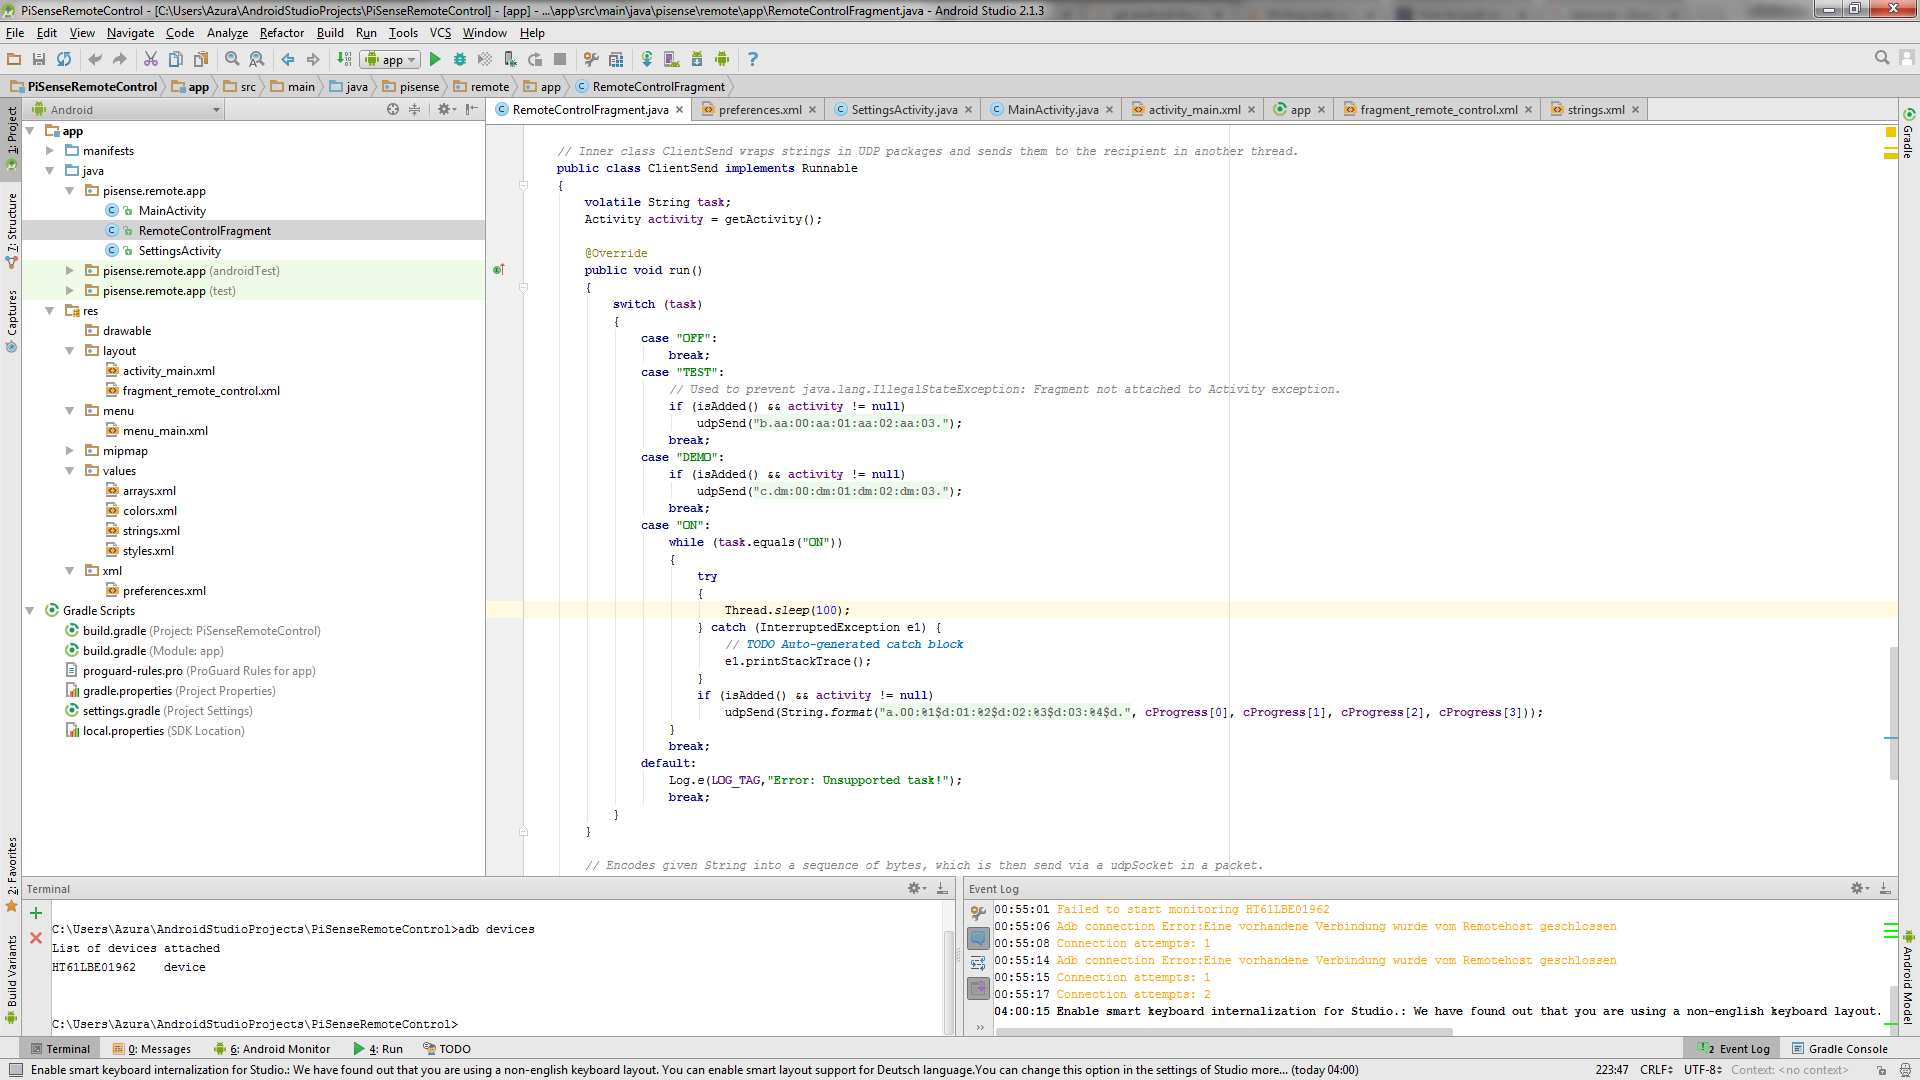
\includegraphics[width=0.9\textwidth]{run.png}
			\caption{Innere Arbeiterklasse ClientSend.\label{run}}
		\end{figure}
		%
		Die volatile String Variable task wird hierbei von der Hauptklasse so manipuliert, dass der gew"unschte Befehl per UDP weiter gesendet werden kann. Die Befehlsketten sind jeweils in der String resource.xml abgespeichert und werden von der udpSend Methode in ihre Byte-Sequenz zerlegt bevor sie als packet weitergeschickt werden.
		\begin{figure}[h!]
			\centering
			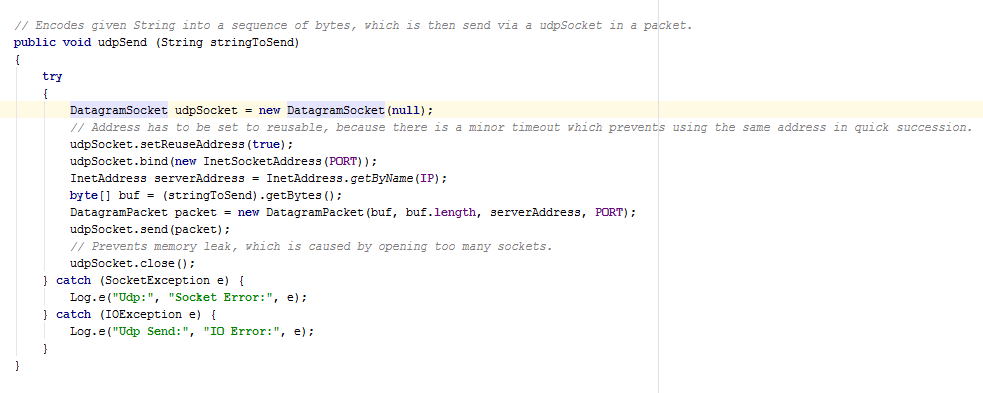
\includegraphics[width=\textwidth]{udp.png}
			\caption{Methode udpSend.\label{udp}}
		\end{figure}
		%
		\newpage
		Da es sich bei der Manipulation der Rotorgeschwindigkeit nicht um statische Daten handelt wurden Klassenvariablen eingef"uhrt, die Ver"anderung des Seekbar Fortschritts unmittelbar abspeichern. Durch das verwenden der String.Format Methode werden Dezimalwerte nachtr"aglich in die Befehlskette eingef"ugt und in einer loop gesendet. Auf diese Weise lassen sich die Rotoren bis zum Abschalten beliebig beeinflussen.
		\begin{figure}[h!]
			\centering
			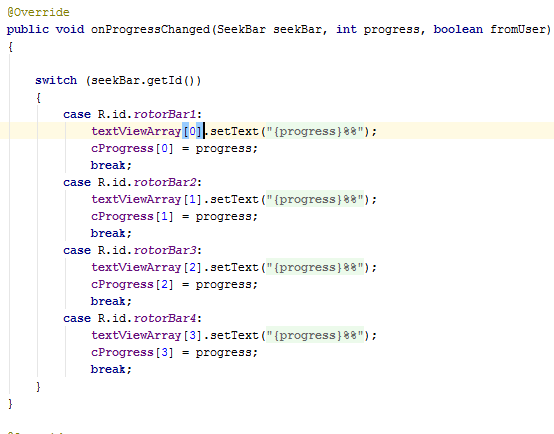
\includegraphics[width=0.8\textwidth]{seek.png}
			\caption{Abspeicherung des Seekbarforschritts in der OnProgressChanged-Methode.\label{seek}}
		\end{figure}
		%
		\newline
		Eine letzte Funktionalit"at der App ist das Abspeichern einer bevorzugten IP-Adresse, sowie eines Ports. Dies erm"oglicht das Verbinden der App auch mit anderen Ger"aten. Es gibt auch einen Default Modus der fest auf die IP und den Port des im Projekt verwendeten Quadrocopters eingestellt ist. Hierbei handelt es sich um eine Checkbox zum de-/und aktivieren. Im Gegensatz zu normalen Layouts bezieht die SettingsActivity ihr Aussehen aus einer preferences.xml. Diese SharedPreferences XML speichert die eingegebenen Einstellungen auch nach verlassen der App.
		\newpage
		\begin{figure}[h!]
			\centering
			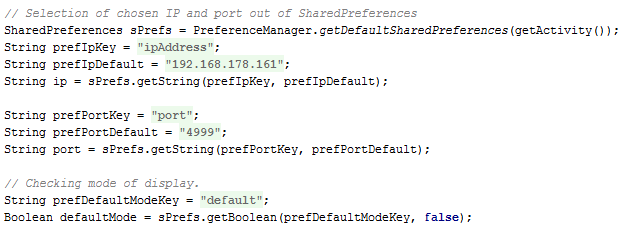
\includegraphics[width=0.8\textwidth]{pref.png}
			\caption{Auslesen der SharedPreferences XML und Pr"ufen auf Darstellungsmodus.\label{pref}}
		\end{figure}
		
			
\end{document}
%
